\section{Introduction}\label{sec:intro}

A grower can plan transport from a calibrated estimate of the number of fruit in a block. A robot updating an inventory on a second pass through a row must recognize fruit it recorded on the first. A census for scheduling oil-palm harvests must assign each bunch to one palm and one harvest window. The last two tasks require an inventory that preserves the identity of each fruit across observations.

Field comparisons show two ways that aggregate measures can hide errors. On 16 mango trees, \citet{stein2016image} found that counts from two sides had a higher coefficient of determination than the estimates from tracking and triangulation ($R^2=0.94$ versus $0.90$), yet systematically underestimated the harvest. In a separate mango video test, \citet{wang2019mango} found that duplicate tracks after occlusion partially offset missed fruit. A calibration therefore needs to account for bias. An evaluation of inventory accuracy also needs to check which fruit were counted.

Earlier reviews explain how detectors respond to occlusion and variable light, how sensors measure fruit, and how imagery supports yield estimation \citep{gong2025fruit,trentin2024tree,fu2020application}. An inventory adds a question that spans these topics. Which observations refer to one fruit? That decision determines how many records can receive a label for size, maturity, or harvestability. It also identifies where methods from tracking and multi-camera re-identification may be of use (Section~\ref{sec:position}).

This systematic review relates six ways of handling repeated observations to the evidence available from video, separate photographs, 3D scans, and repeat visits. Comparisons on shared data show when an additional view expands coverage, when matching reduces duplicates, and when either is obscured by the choice of counting rule or reference. Oil palm brings these problems together. Fronds hide different bunches from each side, and a census must link the observations that show the same bunch before assigning it to a harvest window.

Four questions guide the review. (1) What information does each association mechanism need? (2) Under which conditions do the mechanisms reduce duplicates and misses, and which reference supports that inference? (3) How can several observations of a fruit support one class label? (4) Which parts of an on-palm bunch census have been demonstrated, and what remains to be tested? The remainder of this article is organized as follows. Sections~\ref{sec:method} and~\ref{sec:framework} establish the review and its design space. Sections~\ref{sec:acq}--\ref{sec:palm} examine the evidence from acquisition through association and attribute assignment, with depth and oil palm as applied cases. Sections~\ref{sec:agenda}--\ref{sec:conclusion} draw implications for evaluation and deployment.

\section{Review method}\label{sec:method}

This systematic mapping review uses a configurative synthesis because the studies use different crops, capture protocols, outcomes, and reference counts \citep{petersen2015mapping,grant2009typology}. The review was not registered. Reporting follows the applicable items of the Preferred Reporting Items for Systematic Reviews and Meta-Analyses (PRISMA)~2020 \citep{page2021prisma,page2021elaboration}. Supplementary Section~S5 gives the checklist.

\subsection{Search strategy}
The Scopus Search API was queried on 28 September 2026 (Coordinated Universal Time). Thirteen strings in nine query sets covered fruit counting, oil-palm imaging, class attributes, depth sensing, earlier reviews, and transferable methods. The search covered 2012--2026. For the six searches in the two query sets for methods outside agriculture, the 25 most cited records per search were retained. Appendix~\ref{app:queries} gives the full strings and filters. Supplementary Section~S7 summarizes the queries and their returns. One review identified outside the database search was available online before the search date and assigned to a 2027 volume.

\subsection{Inclusion and exclusion criteria}\label{sec:criteria}
Eligible reports were (i) imaging studies that evaluated counting, yield estimation, detection with a class attribute, localization, or sizing of fruit on plants, (ii) reviews of these topics, or (iii) methods studies relevant to observation or association. Oil-palm mill grading and imaging of loose fruit beneath palms were also eligible. Exclusions covered (i) objects outside this scope, (ii) postharvest or laboratory-only imaging, apart from oil-palm mill grading, (iii) yield modelling without fruit-level observations, (iv) manipulation alone, (v) detection without counting or another qualifying evaluation, (vi) non-imaging sensors, and (vii) records lacking both an English title and an English abstract. Supplementary Section~S1 explains the treatment of records with unavailable abstracts.

\subsection{Study selection}\label{sec:screening}
One reviewer used a large language model to assist with title screening, eligibility assessment on titles and abstracts, and assessment of the available full texts. Decisions that changed a group or excluded a retrieved report were checked against the source. Supplementary Section~S1 gives the screening procedure, agreement on samples, and the identification of \nOther reports outside Scopus. Reports that duplicated the content of an included report were excluded (\nFTExclEight reports). Separate reports using the same data were retained, with shared evidence accounted for during appraisal.

The search for full texts covered \nSought reports. Of these, \nNotRetrieved were unavailable, \nFTAssessed were assessed, and \nFTExcl of the assessed reports were excluded. The map contains \nIncluded reports, including \nScopusIncl from Scopus. Fig.~\ref{fig:prisma} shows the complete flow. Supplementary Data S1 identifies each assessed report and gives reasons for full-text exclusions.

\begin{figure*}[!t]
\centering
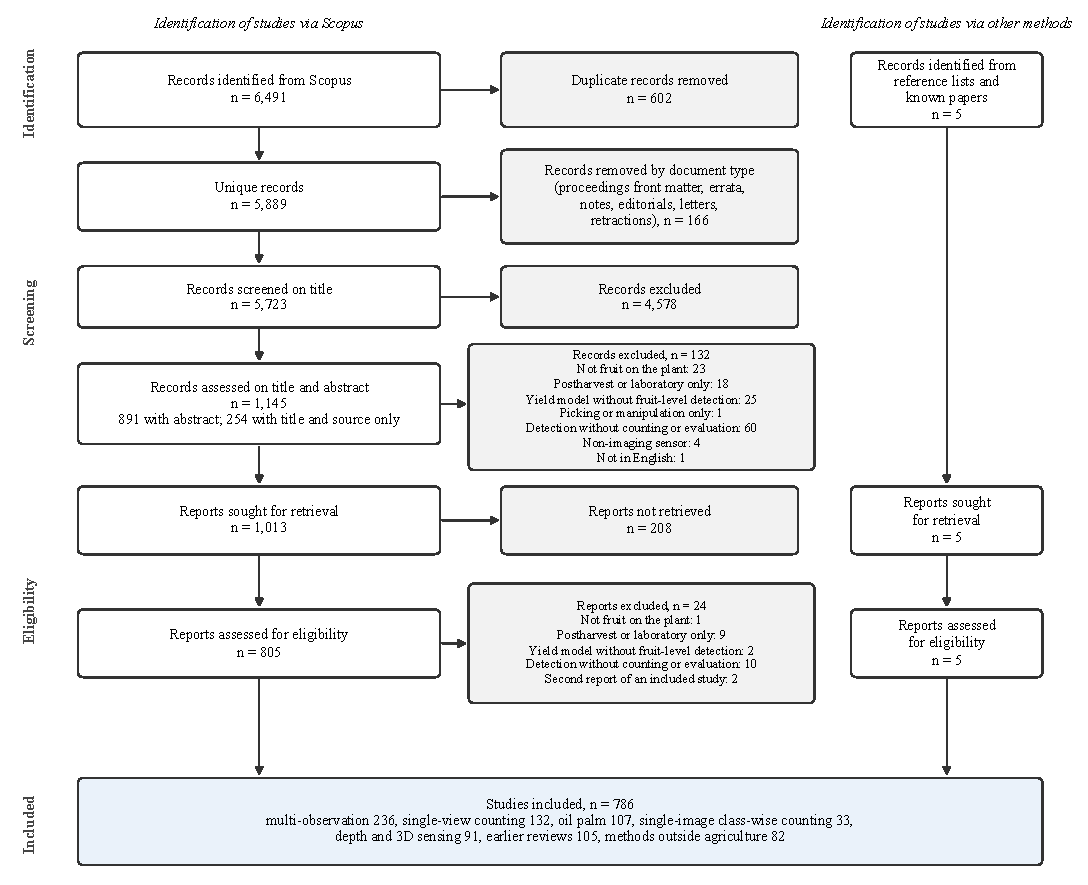
\includegraphics[width=0.88\textwidth]{F01_prisma}
\caption{Record identification, screening, and full-text assessment.}\label{fig:prisma}
\end{figure*}

\subsection{Data extraction and coding}\label{sec:coding}
The map assigns each report to one of seven groups according to its role in the synthesis (Supplementary Sections~S2 and S7). The multi-observation records were coded from the full text for acquisition, association mechanism, class assignment, principal result, count reference, and outcome level. The oil-palm records were coded for task, setting, modality, views, and instance-level classes. Supporting groups were classified at full-text eligibility, with descriptive keyword codes spot-checked. A report can contribute to the frequency of more than one association mechanism. Appendix Table~\ref{tab:c1matrix} provides one evidence row per multi-observation report.

\subsection{Appraisal and synthesis}\label{sec:appraisal}
The main comparisons use the same test images, videos, or plants and report an outcome for every arm. To attribute an effect to one component, a comparison must hold the other components and the reference fixed. Where several components changed, the result describes the change to the combined pipeline. Detector-only comparisons address observation-stage performance. The synthesis interprets values against the reference used in each test and reports them without pooling.

Appraisal distinguishes annotated imagery from field references, tests on shared data from results reported on different data, and methods evaluated by their developers from comparisons favouring alternatives. The stated rule for high, moderate, or low certainty uses independent groups, crop coverage, reference counts, and conflicting results. Supplementary Section~S7 gives that rule. Reports from one research group or on the same data do not provide independent confirmations. Grades apply to findings. The review used no formal study-level risk-of-bias tool.

\section{What constitutes a fruit inventory?}\label{sec:framework}

An observation is a measurement in one image or frame. A fruit record is a hypothesis that one or more observations belong to a single physical fruit. A plant inventory is a set of these records assigned to a named plant, with a count and any class attributes of interest. Fig.~\ref{fig:kerangka} connects these outputs. Acquisition makes fruit observable. Detection or segmentation describes what is visible. Association groups repeated observations. Attribute assignment determines the label of a record, and inventory aggregation assigns records to plants and totals them. A system can be accurate at an earlier stage while the next stage fails.

\begin{figure*}[!t]
\centering
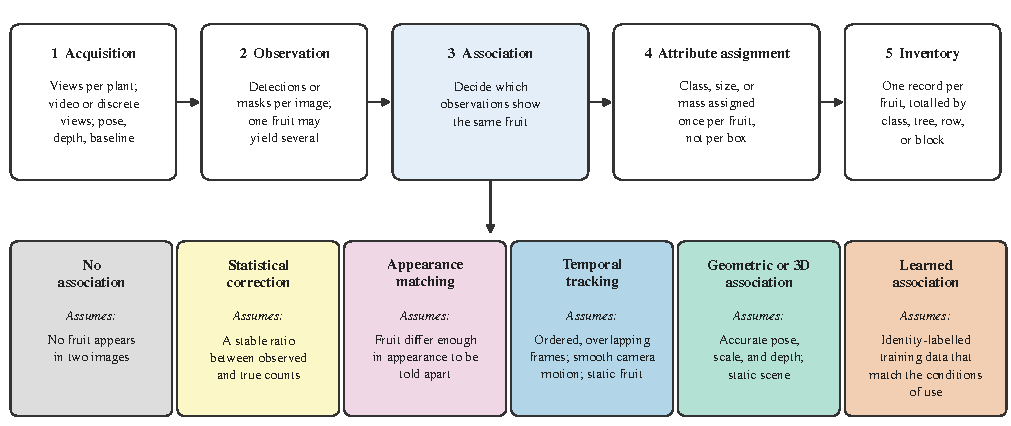
\includegraphics[width=0.88\textwidth]{F03_kerangka}
\caption{Five stages linking image acquisition to an inventory of unique fruit by class.}\label{fig:kerangka}
\end{figure*}

\subsection{Duplicates, missed fruit, and the reference}\label{sec:dupsources}
A fruit can be counted repeatedly in consecutive frames, after leaving and returning to view, or in views acquired on different sides or visits. Those errors differ in the information available to resolve them. Short-term motion is informative in consecutive frames. It becomes less informative after long occlusion and cannot establish correspondence by itself across independently acquired passes. A plant count can also omit fruit because they are hidden from every view, because a detector never finds them, or because the association stage merges them with their neighbours.

Let \(N_{\mathrm{field}}\) be an independent field count, \(N_{\mathrm{vis}}\) the number of unique fruit verified in the acquired views of the same plants at the same time, and \(\widehat N\) the number of predicted records. Under a one-to-one match to visible reference fruit, \(U\) predicted records and \(L\) reference fruit are unmatched. The signed errors are
\begin{align}
\widehat N-N_{\mathrm{vis}} &= U-L,\\
\widehat N-N_{\mathrm{field}} &= U-L-(N_{\mathrm{field}}-N_{\mathrm{vis}}).
\label{eq:count-gap}
\end{align}
The unmatched records can be splits of real fruit or background detections, and the unmatched visible fruit can be detection misses or losses under erroneous merges. When both references are complete and refer to the same crop unit, the last term measures the coverage lost at acquisition. Fig.~\ref{fig:inventory-error} illustrates one duplicate cancelling one miss among visible fruit, while two fruit remain hidden from every view. The signed error is zero against the visible reference and minus two against the field reference.

\begin{figure*}[!t]
\centering
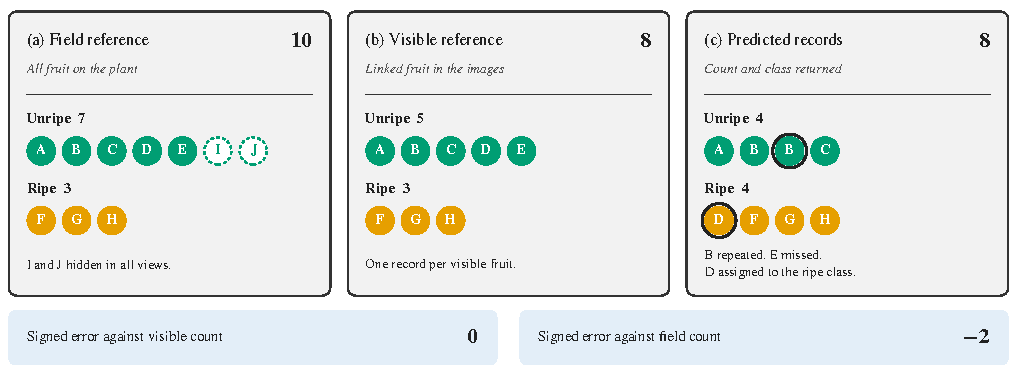
\includegraphics[width=\textwidth]{galat-inventaris}
\caption{Illustrative inventory with errors that cancel in the visible count. Each letter identifies one fruit. Dashed outlines mark hidden fruit. Solid outer rings mark the extra record of B and the class reassignment of D.}\label{fig:inventory-error}
\end{figure*}

The association stage can also be isolated using annotated observations. If every visible fruit contributes at least one observation, every observation belongs to a true fruit, and all observations are assigned to predicted groups, each true fruit that touches \(k\) predicted groups contributes \(k-1\) extra fragments. A predicted group that joins observations of \(j\) true fruit contributes \(j-1\) lost identities. The sum of excess fragments minus the sum of lost identities equals \(\widehat N-N_{\mathrm{vis}}\). Reporting both detects cancellation. An experiment with estimated detections needs to report detection misses and spurious observations as well, or repeat the association test with the annotated inputs.

\subsection{Six ways to handle repeated observations}\label{sec:mechdefs}
A system with \textit{no association} assumes that each fruit enters the count once by construction, for example through non-overlapping sampling or an external tag. \textit{Statistical correction} estimates an aggregate from observed counts without identifying duplicates. Four other families make a decision about individual observations. \textit{Temporal tracking} uses continuity between ordered frames. \textit{Appearance matching} uses visual similarity and typically narrows the candidate set with motion or position. \textit{Geometric or 3D association} projects observations into a shared frame or forms a composite representation in which a fruit can be localized once. \textit{Learned association} estimates correspondence using training examples or learned features. These mechanisms can operate together. Appendix Table~\ref{tab:c1matrix} records the combinations used in the included studies.

\subsection{Acquisition and mechanism are coupled}\label{sec:landscape}
Video provides continuity along a path. Discrete views trade that continuity for a wider baseline. Scans provide a spatial representation, and repeated sessions add the possibility of genuine changes in the crop. Of the \nMethod multi-observation method studies, \nVideo use video, \nDiscrete use discrete views, \nScan use 3D scans, and \nRevisit link observations across visits. Geometry appears in \nDiscreteGeom and statistical correction in \nDiscreteStat of the discrete-view studies, with overlapping membership where a study combines mechanisms. These frequencies describe how methods have been used, rather than which method is most accurate. Supplementary Section~S8 shows the full distributions and how they changed over time.

\section{Acquisition: what enters the inventory}\label{sec:acq}

Acquisition determines both the fruit available to count and the evidence available to link it. A single frame may suffice for a count of visible fruit, or for a calibrated estimate under a stable canopy. A second frame changes the problem when it reveals both new fruit and fruit already seen. Table~\ref{tab:acq} gives comparisons on the same plants or bunches. The effect of adding a view depends on whether it brings new coverage, repeats existing evidence, or does both.

\begin{table*}[!t]
\centering
\caption{Acquisition comparisons on the same plants or grape bunches.}\label{tab:acq}
\footnotesize
\begin{tabularx}{\textwidth}{@{}L{2.6cm}L{1.6cm}L{2.9cm}YL{2.4cm}@{}}
\toprule
Study & Crop, scale & Designs compared & Reported result & Count reference\\
\midrule
\citet{stein2016image} & Mango, 16 trees & One image of one side; one image per side; multi-view tracking with triangulation (tracking + geometric) & Fitted count-to-harvest slopes: 0.27 (single, $R^2=0.81$), 0.54 (dual, $R^2=0.94$), 1.014 (multi-view, $R^2=0.90$) & Harvest count\\
\citet{wang2019mango} & Mango, 21 trees & One image per side; video tracking & 40\% of harvest (bias-corrected RMSE 21.7 fruit/tree) vs 62\% (RMSE 18.0) & Harvest count\\
\citet{payne2013estimation} & Mango, 15 trees & Manual count in one image per side; two opposing sides summed; four sides summed & Mean 38.1--45.7 fruit per side, 77.4--89.9 for two sides, 167.3 for four sides, against 61.7 per tree; $R^2=0.81$--0.93 in every arm & Hand count per tree\\
\citet{mirhaji2021fruit} & Orange, 100 trees & Two sides summed; four sides summed; two or four sides chosen by canopy size & Best MAPE over three detectors 48.6\% (two sides), 15.0\% (four sides), 9.4\% (by canopy size); four sides overestimated thin canopies & Harvest count per tree\\
\citet{gongal2016apple} & Apple, tall spindle & One side; both sides with 3D duplicate removal (geometric association) & Crop-load estimation accuracy 58\% vs 82\%; error in identifying duplicate apples 21.1\% & Manual count\\
\citet{qureshi2023seeing} & Apple fruitlets, 10 branch scans & One-sided vs two-sided scans from an over-canopy robot & Counting accuracy 73.7\% vs 81.17\% & Manual count\\
\citet{li2025field} & Blueberry, 26 plants & Top view; top, left, and right views combined by regression on per-view counts & Each view showed 47.3--53.87\% of the harvested berries; $R^2=0.71$ (top) vs 0.73, MAPE 23.1\% (three views) & Harvest count per plant\\
\citet{zhang2022complete} & Holly, 614--753 fruit per tree & UAV circling the tree at eight radii (0.6--2.0~m); views stitched into one panorama & Fruit captured in the panorama 99.19\% at 0.6~m and 92.53\% at 2.0~m; counted 98.53\% and 90.37\% of all fruit & Hand count of all fruit on the tree\\
\citet{rist2018high} & Grape, 48 bunches & One-side scan in the field or laboratory vs 360$^\circ$ scan, structured-light 3D scanner & Mean berries per bunch 66 (each one-side scan) vs 137 (360$^\circ$); berry diameter 12.8--13.3~mm in all & Destructive berry count\\
\citet{arizasentis2025comparative} & Grape, commercial vineyard & Single-view vs multiple-view UAV video with tracking & Tracked/ground-truth ratio 13--23\% vs 27--74\% across trials; multi-view tracking degraded by motion blur & Annotated video\\
\citet{felippomes2026video} & Apple, 420 trees & Two RGB-D sensors, three distances, two dates, one or both sides & Best MAPE 6.91\%, $R^2=0.733$ at 225~cm; both sides reduced RMSE per stretch & Harvest count per 5~m stretch\\
\citet{vijayakumar2023tree} & Citrus, per tree & UAV features plus fruit counts from one or two sides & MAPE 23.45\% (one side) vs 25.72\% (two sides), both better than UAV only (35.59\%) & Harvest per tree\\
\bottomrule
\multicolumn{5}{@{}p{\textwidth}@{}}{\rule{0pt}{2.6ex}\textit{Note:} Values are as reported by the authors, with fractions given as percentages. Count references and metrics differ between rows, so values should be compared only within a row. MAPE, mean absolute percentage error; RGB-D, red-green-blue-depth; RMSE, root-mean-square error; UAV, unmanned aerial vehicle.}
\end{tabularx}
\end{table*}

\subsection{What a single view can measure}\label{sec:single-view}

The target in a single image can be a visible instance, a density integral, or an estimate of a larger unit such as a bunch, tree, or block. These outputs require different supervision and support different uses. A method that produces one point per visible berry can locate candidates for thinning. A model that predicts how many berries are hidden can inform crop load. The prediction of a hidden berry contributes to a total but gives no observed identity to link.

Count error can conceal missed fruit and false detections even in a single image. In one illustrated citrus comparison, \citet{zhang2019fast} used colour separation and a Hough transform to return 113 detections against a manual count of 117. Seven fruit were missed and three background features were counted. The difference of four therefore concealed ten errors. In apple canopies, \citet{bhattarai2024agregnet} estimated fruit density from point annotations and obtained a mean absolute error (MAE) of 3.1 fruit per image and a root-mean-square error (RMSE) of 4.0 on their fruit image test set. A branch dividing the visible surface of one apple into three parts produced three density peaks in one example. Point supervision reduced the need to label boundaries, but the method could still split an occluded fruit within one image.

Cluster membership adds a second ambiguity. A berry can be detected correctly and assigned to the wrong bunch. \citet{xie2026unified} paired berry points with predicted cluster masks in annotated vineyard images and tested the pipeline by replacing individual stages with reference inputs. Providing reference cluster detections and prompt geometry reduced the all-cluster penalized mean relative deviation from 0.5062 to 0.1289. Replacing the berry points alone reduced it to 0.4783. Under that protocol, missing or poorly localized clusters mattered more than the remaining berry-point error. Both image sources contributed to training and evaluation. The result concerns assignment of visible berries in those images, with hidden berries and independent vineyard transfer outside the test.

An accurate count of visible fruit can still sample only a small share of the crop. \citet{zhang2024open} used blueberry imagery to estimate maturity and a proxy for yield across phenotyping environments. They cautioned that their detector captured about a quarter of total yield and was trained with images from one plant type and collection period. In grapevine images, \citet{victorino2020yield} recorded 4.3--6.3 visible bunches per metre in sunlit views of non-defoliated vines, against 11.8--12.1 bunches per metre counted in the field. The gap belongs to the visibility and sampling problem. A different detector operating on the same pixels cannot supply evidence of completely hidden fruit.

\subsection{When additional views help}\label{sec:repeat-views}

Opposed views help when the new surface contains fruit absent from the first view. In the 16-tree mango comparison of \citet{stein2016image}, the fitted count-to-harvest slope increased from 0.27 to 0.54 with a second side. Replacing the detector output with hand labels raised the two-view slope to 0.64, leaving substantial undercoverage even with better observations in those frames. By contrast, \citet{payne2013estimation} counted 167.3 visible fruit on average when four views were summed across 15 mango trees, although the mean manual tree count was 61.7. The four-view total still tracked the differences between trees. A high correlation can survive a large systematic bias in either direction.

Canopy structure controls the trade-off. \citet{mirhaji2021fruit} obtained a mean absolute percentage error (MAPE) of 48.6\% from a two-side orange count and 15.0\% from four sides on the same trees, with a canopy-dependent choice giving 9.4\%. Four sides tended to overestimate thin canopies. \citet{silwal2016hierarchical} found the complementary pattern in shallow tall-spindle apple canopies: 38 of 1{,}827 fruit were missed, whereas 130 false positives remained, mainly because real apples were counted again. The useful question is how many distinct fruit each added view reveals relative to how many existing fruit reappear.

The distinction becomes sharper when added views are linked. On 21 dense-canopy mango trees, \citet{wang2019mango} recorded 40\% of the harvested fruit from an image on each side and 62\% with video tracking. Across three apple datasets, \citet{hani2020comparative} found that a plain sum of opposing sides returned 103.86--147.81\% of the harvest reference with a fixed detector, whereas a geometric merge returned 95.56--97.83\%. These comparisons distinguish increased coverage along a pass from the removal of duplicates across passes. In the citrus models of \citet{vijayakumar2023tree}, adding a second side did not significantly reduce per-tree error ($p=0.29$). The value of the second side depends on its coverage and on how the pipeline handles overlap.

\subsection{Capture protocols for different tasks}\label{sec:acq-protocol}

Video along a row provides small changes between neighbouring frames. Independently taken views around a plant cover larger angular gaps, but give no observations during the change of viewpoint. A panorama or 3D scan can resolve some of those gaps if the images share enough features to register. \citet{zhang2022complete} stitched views taken around holly trees into a panorama. The share of manually counted fruit recorded in the panorama fell from 99.19\% at a flight radius of 0.6~m to 92.53\% at 2.0~m. In that setting, increasing the radius reduced the share of fruit retained in the reconstruction. Simulation and artificial-tree studies of active view selection address the corresponding planning problem, with limited evidence on independent field counts \citep{roy2017active,zaenker2021viewpoint,zaenker2023graph}.

The need for coverage also depends on the output. On the same grape bunches, \citet{rist2018high} reported a mean of 66 berries in one-sided scans and 137 in full-circle scans, whereas mean berry diameter stayed between 12.8 and 13.3~mm across capture modes. A view set adequate for a size summary may be inadequate for a count of the same object. Tests of new capture protocols should therefore report the incremental number of unique reference fruit acquired at each step, together with the number seen again. Fig.~\ref{fig:hasil}a compares acquisition and linking outcomes against the reference used within each study. The mango slopes reported by \citet{stein2016image} are plotted as percentages. The other studies report ratios to field or video counts. The comparison within each study matters because the references differ.

\begin{figure*}[!t]
\centering
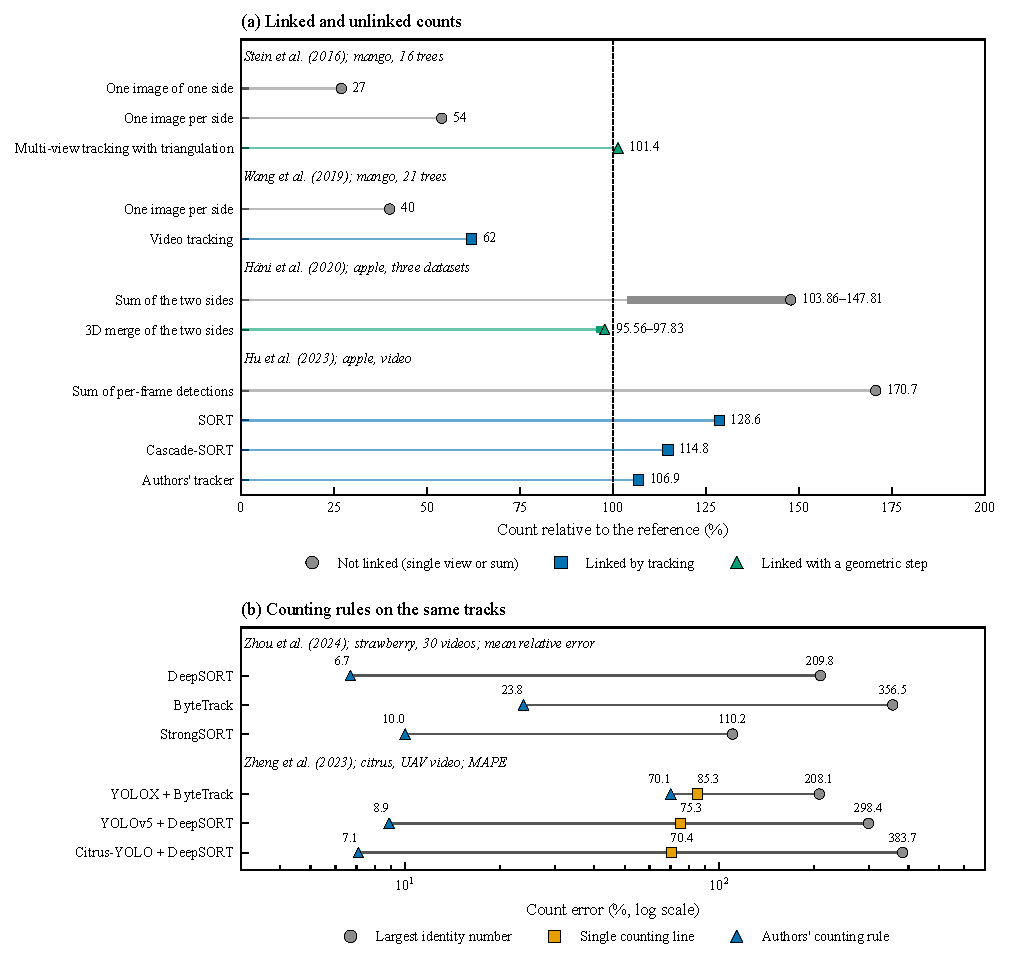
\includegraphics[width=0.86\textwidth]{F12_hasil}
\caption{Within-study comparisons ($n=6$ studies). (a) Counts relative to their references. The values from \citet{stein2016image} are fitted count-to-harvest slopes multiplied by 100. Thick bars show the range over three datasets, and the dashed line marks equality with the reference. (b) Count error under different rules applied to the same tracks, on a logarithmic scale.}\label{fig:hasil}
\end{figure*}

Where repeated views are necessary, the next decision is how to combine them. A calibration can adjust the expected total. Claiming that a particular fruit has already been seen requires correspondence evidence (Section~\ref{sec:mech}).

\section{Evidence by association mechanism}\label{sec:mech}

The usefulness of an association cue depends on how the images were acquired. Motion helps when observations are close in time. Appearance can distinguish fruit when the visible patches differ enough, and geometry can connect observations that share a coordinate frame. Table~\ref{tab:mechsyn} sets out those assumptions. Table~\ref{tab:assoc} shows what changed when specific pipeline components were compared on shared test data. Some comparisons isolate a component. Others change several steps together. Their count and identity outcomes answer different questions. Supplementary Section~S9 provides the broader comparison record, and Appendix Table~\ref{tab:c1matrix} lists each multi-observation report.

\begin{table*}[!t]
\centering
\caption{Association mechanisms: assumptions, duplicate sources removed, reported failure conditions, evidence on the same data, and applicability to a few discrete views.}\label{tab:mechsyn}
\footnotesize
\begin{tabularx}{\textwidth}{@{}L{2.0cm}L{2.9cm}L{2.2cm}YL{3.0cm}L{2.3cm}@{}}
\toprule
Mechanism & Assumes & Duplicate sources removed & Reported failure conditions & Strongest same-data evidence & Few discrete views\\
\midrule
No association & Each fruit contributes one count by design & None & The same fruit appears more than once in the count & No direct comparison & When sampling prevents repeat counts\\
Statistical correction & A stable ratio between observed and true counts & None individually; absorbed on average & Change of orchard, canopy, season, or acquisition \citep{anderson2021estimation,koirala2021attempting,islam2022ground} & Occlusion factor raised the absolute percentage error against packhouse counts from 11\% to 17\% in nine mango orchards \citep{anderson2021estimation}; learned correction did not hold in the next season \citep{koirala2021attempting} & Applicable; refit per orchard and season\\
Temporal tracking & Ordered, overlapping frames; smooth camera motion; static fruit & Consecutive frames; re-entry only within the track lifetime & Low frame rate, camera shake, long occlusion, second side of the row \citep{qi2025assessment,wei2025multi,saraceni2024agrisort,wang2019mango} & In apple video, summing detections gave 495 and tracking gave 310 against a manual count of 290 \citep{hu2023fruit} & Within a pass with overlapping frames\\
Appearance matching & Fruit differ enough to be told apart & With motion or position: re-entry & Look-alike fruit, frame-rate drops, class appearance changing under occlusion, fruit texture changing between sessions \citep{genemola2023video,qi2025assessment,kirk2021robust,mirbod2021field} & A generic descriptor outperformed motion matching (SORT) but not consistently a tracker that keeps low-confidence boxes (ByteTrack); fruit-specific cues gained in the authors' own tests (Table~\ref{tab:assoc}) & Untested as the only cue\\
Geometric or 3D association & Reliable spatial registration and a scene stable enough for matching & All three, including the second side & Missing frames, time-sync error, platform oscillation, fruit clusters, misaligned sides, noisy poses \citep{stein2016image,genemola2020fruitb,qureshi2023seeing,meyer2025fruitnerf} & Tracking plus 3D correction cut the summed absolute count error on oranges from 593 to 203 \citep{liu2018robust}; 3D merge vs sum of sides \citep{hani2020comparative} & Applicable if pose can be estimated across wide baselines\\
Learned association & Features or training examples that distinguish repeat observations & Depends on training & Pose error in re-identification, occlusion splitting instances \citep{santos2026multi,meyer2025fruitnerf} & FruitNeRF++ reached F1 0.765 on an apple benchmark. The fruit-specific comparator reported 0.881 on the same dataset \citep{meyer2025fruitnerf} & Evaluate with cross-view identity labels\\
\bottomrule
\multicolumn{6}{@{}p{\textwidth}@{}}{\rule{0pt}{2.6ex}\textit{Note:} The three sources of double counting are the same fruit in consecutive images, a fruit lost and picked up again as a new track, and a fruit seen from both sides of the plant (Section~\ref{sec:dupsources}). SORT, simple online and realtime tracking.}
\end{tabularx}
\end{table*}

\begin{table*}[!t]
\centering
\caption{Selected contrasts on shared test data, with the reference and the part of the system changed.}\label{tab:assoc}
\footnotesize
\setlength{\tabcolsep}{4pt}
\begin{tabularx}{\textwidth}{@{}L{2.6cm}L{3.4cm}YL{3.5cm}@{}}
\toprule
Choice and study & Test and reference & Reported contrast & What the contrast supports\\
\midrule
(1) Appearance under missed detections \citep{villacres2023apple} & Apple video with annotated boxes subsampled to 60\% & Multiple-object tracking accuracy (MOTA) was 13.8\% with SORT and 69.3\% with DeepSORT & A descriptor helped recover from artificial detection gaps in this test\\
\addlinespace
(2) Tracker under a fixed detector \citep{qi2025assessment} & Tomato clusters at 30 frames/s with the RT-DETR detector, against annotated tracks and manual video counts & MOTA was 84.3\% for DeepSORT and 83.5\% for ByteTrack. Relative count accuracy was 87.6\% and 95.5\%, respectively & The two metrics ranked the same tracker pair differently\\
\addlinespace
(3) Geometric correction after tracking \citep{liu2018robust} & Visible oranges per tree and apples per row segment, with human image labels & Adding 3D duplicate and outlier rejection reduced summed absolute error from 593 to 203 oranges and from 673 to 322 apples & Both duplicate removal and spatial filtering changed the count\\
\addlinespace
(4) Merging the two sides of a row \citep{hani2020comparative} & Three apple datasets, against harvested counts, with the ResNet50 detector & Summing both sides returned 103.86--147.81\% of the reference. Merging in 3D returned 95.56--97.83\% & Merging brought counts closer to harvest with the detector held fixed\\
\addlinespace
(5) Registration across dates \citep{yoshida2026cross} & 49 initially detected and verified grape clusters, matched across three weeks & 34 clusters (69.39\%) retained the correct correspondence with branch registration versus none with centroid normalization alone & Registration helped among detected clusters. Growth and occlusion still caused failures\\
\addlinespace
(6) Track-to-count rule \citep{zhou2024advancing} & 30 strawberry videos with annotated counts & For DeepSORT, mean relative error fell from 209.8\% to 6.7\% with the authors' counting rule. For StrongSORT it fell from 110.2\% to 10.0\% & The counting rule reversed the ranking for these two trackers\\
\addlinespace
(7) Statistical correction \citep{anderson2021estimation} & Nine mango orchards with comparable methods, against packhouse totals & Mean absolute percentage error rose from 11\% for raw multi-view counts to 17\% after correction with an occlusion factor & A fitted correction can worsen agreement with orchard totals\\
\addlinespace
(8) Summing detections or linking them \citep{hu2023fruit} & Apple video, against 290 manually counted fruit & The sum of detections was 495. The authors' tracker returned 310 & Tracking reduced the overcount, with a residual whose sign alone does not identify the errors\\
\bottomrule
\end{tabularx}

\smallskip
\parbox{\textwidth}{\rmfamily\footnotesize\textit{Note:} Values are as reported. The rows differ in crop, scale, and reference. Comparisons are interpreted within each row. SORT, simple online and realtime tracking. RT-DETR, real-time detection transformer.}
\end{table*}

\subsection{No association and statistical correction}\label{sec:mech-stat}
An aggregate calibration can be useful when the relationship between observed and reference counts holds on new plants. It does not assign identities to repeated observations. Statistical correction appears in \nStat of \nMethod method studies. The one method coded as no image-based association used physical tags to supply bunch identities \citep{kassim2012oil}.

Calibration can follow linking when the aim is to convert a count of visible fruit into a yield estimate. \citet{nuske2014modeling} registered images from a vehicle driving along vineyard rows and related berry counts to harvest yield. Because the berries were first linked by registration, the study is counted under geometric association, and only its calibration step belongs here. Total yield was within 4\% of harvest with calibration from a previous harvest, and within 3\% with destructive samples taken at imaging.

Calibration can yield a useful orchard total even when the images capture only a fraction of the crop. \citet{linker2015estimation} tested this approach on apple trees, photographing 42 trees from two sides at three heights. The detections in the six images of a tree corresponded to about one third of its yield. After calibration on 14 trees, the overall estimate for the 42 trees was within 10\% of the actual yield, although single-tree errors were sometimes large. The authors described the result as a self-calibrating system that would need the grower to count 15--20 trees. In a different approach, \citet{song2014automatic} mapped repeated observations of pepper fruit to common coordinates and grouped them with a statistical clustering step. Regression from partial views remains common in UAV work \citep{apoloapolo2020cloud,li2023blueberry}.

An accurate orchard total can conceal substantial errors on individual trees. \citet{linker2017procedure} extended the apple design to four night-time datasets imaged at three camera heights and combined the counts of two to six images per tree in multiple linear models. The best models estimated total yield within 10\% of the harvest, but the standard deviation of the single-tree error was about 26--37\% of the mean tree yield. Images from three cameras were only slightly better than images from two, and images of one side of the tree did not make the estimate markedly worse.

A calibration fitted to one set of trees can worsen aggregate estimates. A close correlation on the calibration data is insufficient to establish transfer. \citet{anderson2021estimation} found that correcting multi-view counts with an occlusion factor from hand-counted trees did not improve the estimate in 16 of 20 mango orchards and increased the average error from 11\% to 17\% in the nine orchards with all methods. The error on trellised canopies (25.2\%) was several times that on other canopy systems (3.4--8.2\%).

Performance on the plots used for fitting provides little evidence that a visibility model will hold in a new season. \citet{koirala2021attempting} tried to replace the factor with a model of hidden fruit learned from canopy features. The model reached $R^2=0.98$ against the harvest counts of 98 trees in its training season, but no visual feature correlated with the number of hidden fruit, and the models did not hold in the following season. Image features predicted the hidden share in a narrower setting: \citet{victorino2022overcoming} estimated the visible share of grape bunches (16--64\%) from canopy porosity and visible bunch area, with $R^2=0.80$ on a validation set drawn from the same vineyard plots.

The factor also changes with canopy architecture within one site. \citet{islam2022ground} fitted a separate calibration factor to grader counts at harvest for each training system of four stone-fruit crops, with factors from 0.796 to 3.875. Two peach systems alone required factors of 1.882 and 3.295. \citet{payne2014estimating} applied one two-side imaging protocol to mango in two orchards and seasons, and the summed image counts held 84\% of the tree count with $R^2=0.51$ on 50 trees in the first and 59\% with $R^2=0.92$ on 21 trees in the second. \citet{linker2018machine} transferred an apple detector between two years with different cameras and lighting, but the count adjustments fitted on one year were slightly worse than no adjustment on the other.

Two-side counts of mango show the same dependence on the tree. \citet{koirala2019deep} multiplied the detections from both sides of each tree by an orchard factor fitted on about 18 hand-harvested trees. The factors ranged from 1.05 to 2.43 across five orchards, and the orchard estimates differed from packhouse counts by 4.6--15.2\%. The authors attributed the largest error, in the orchard with small trees, to fruit visible from both sides and counted twice. \citet{sarron2020machine} summed the detections in two opposite images of each tree in Senegal and fitted one regression per cultivar ($R^2=0.90$--0.93), with a relative RMSE of 14\% on 52 validation trees, although the F1 score of the pixel classifier fell from 0.73 in a uniform orchard to 0.48 across heterogeneous orchards. Taken together, one fitted factor absorbs both hidden and doubly counted fruit, so its value depends on canopy size, cultivar, and orchard.

The factor also depends on the light at the time of imaging. \citet{denarda2024shd} photographed the east and west sides of 100 super-high-density olive trees under sun and under cloud, and derived a scale factor from hand counts on both sides of five trees: 3.18 for sunny and 2.20 for cloudy images, because more olives were visible under cloud. Against estimated harvest counts rescaled using these factors, the RMSE of the per-tree count before harvest was 462.32 olives in sunny and 875.90 in cloudy images. The study therefore needed one factor for each sky condition, and the condition that made more fruit visible to the hand count gave the larger error for the detector.

Within one orchard, one method was evaluated in seasons it had not been trained on. \citet{apoloapolo2020deep} trained a recurrent network on fruit counts from UAV images of the two faces of 20 orange trees, left out one of three seasons in turn, and estimated the total yield with a mean error of 7.22\%, against 13.74\% for a technician's estimate. Some studies limit duplicates by acquisition instead, either by subtracting the fruit at the corners of eight direction frames, each of which appears in two neighbouring frames \citep{nenavath2024tree}, or by projecting fruit between the cameras of a calibrated rig \citep{villacres2024assessing}.

Statistical correction can therefore serve as a baseline for crop-load forecasting. Its error should be measured on plants held out at the scale of intended use, with particular attention to changes in canopy and visibility. It cannot establish which fruit was counted twice. A system that makes that claim requires linked observations (Section~\ref{sec:agenda}).

\subsection{Temporal tracking}\label{sec:mech-track}
Temporal tracking is effective when consecutive frames keep the fruit close to its predicted image position. A gap in the detections consumes part of the time for which the filter can carry an identity. Tracking appears in \nTrack of \nMethod method studies (Supplementary Section~S8). Most use tracking by detection. A detector finds fruit in each frame, a filter predicts where each track should appear, and an assignment step links detections to tracks. Simple online and realtime tracking (SORT) illustrates this approach \citep{bewley2016simple}. ByteTrack uses low-confidence detections to continue plausible tracks \citep{zhang2022bytetrack}.

\textit{(1) The motion model and the frame rate.} When fruit are stationary during a pass, their displacement between images is largely due to camera motion. \citet{saraceni2024agrisort} estimated that motion from optical flow and removed velocity terms from the tracking filter because projected motion on rough vineyard terrain was nonlinear. SORT lost almost all identities in their sequence with rapid nonlinear camera motion. The frame rate determines how often observations can correct the filter. \citet{wei2025multi} reported that random filter initialization at five frames per second degraded the tracks unless initial velocities were adjusted for each dataset. \citet{qi2025assessment} found that tracking accuracy on tomato video fell as the frame rate was reduced. Camera-motion compensation also addressed shake on a legged robot \citep{zhang2024stablesort} and large displacements in low-frame-rate aerial video \citep{xieli2025pinesort}. A moving fruit adds a separate source of displacement, as the picking experiment of \citet{lou2024online} showed with artificially disturbed citrus.

\textit{(2) Which failure the tracker is built to repair.} Appearance cues can help reconnect a track after a missed detection, but their value depends on the available appearance and motion evidence (Table~\ref{tab:assoc} and Supplementary Section~S9). Against plain motion matching, a re-identification descriptor usually helped. \citet{piazolo2026enhanced} counted grape bunches in UAV video with a counting accuracy of 95.2\% for DeepSORT against 32.7\% for SORT, with mean identity-switch counts of 17.05 and 73.50, respectively. \citet{villacres2023apple} removed annotated apple boxes at random and found that the descriptor mattered once detections went missing: with all boxes the two trackers were close (MOTA 93.0\% and 94.6\%), whereas with 60\% of boxes DeepSORT kept 69.3\% and SORT fell to 13.8\%. On annotated apple boxes, DeepSORT had the lowest MOTA of four trackers on all four datasets \citep{matos2024tracking}, and on litchi a generic re-identification network performed about as well as overlap matching \citep{lu2025iot}.

The advantage of an appearance descriptor was less consistent when the comparator also retained low-confidence detections. On apples, ByteTrack reached MOTA 68.17\% at about 15~ms per image, against 57.35\% for DeepSORT at 128~ms, and the authors attributed the absence of a gain to the similar appearance of apples \citep{genemola2023video}. On tomato clusters, BoT-SORT with re-identification reached the highest MOTA at a constant frame rate (84.6\%), but ByteTrack gave the highest counting accuracy (95.5\%), and the re-identification trackers degraded more when the frame rate varied \citep{qi2025assessment}.

The detector can also change a tracker's count error in a way that a single-image metric fails to predict. In \citet{villacres2023apple}, the detector with the higher AP50 on its validation material gave the larger count error with DeepSORT on the orchard videos. Relative count error was 31.5\% with Faster R-CNN and 20.1\% with YOLOv5, while their detector validation AP50 values were 75.13\% and 72.67\%, respectively. Detection and counting were measured on different material. The comparison shows why selecting a detector by validation AP alone leaves the behaviour of the complete system uncertain.

These methods address different failures. An appearance descriptor can reconnect a broken track. ByteTrack keeps some detections that would otherwise be discarded. Camera-motion compensation corrects the position predicted by a filter on a moving platform. Few studies report detection gaps, frame rate, and motion alongside their count errors. DanceTrack provides an example of an evaluation built around ambiguous appearance and unpredictable motion outside agriculture \citep{sun2022dancetrack}.

\textit{(3) The counting rule can reorder trackers.} A counter that accepts a new track as a new fruit counts a fragment if that identity is reinitialized. Taking the largest identifier also counts any unused identifiers below it. \citet{zhou2024advancing} counted strawberries in 30 videos. The largest-identifier rule gave mean relative errors of 110.2--356.5\% across three trackers. Mapping identities to a counter reduced them to 6.7--23.8\% and replaced StrongSORT with DeepSORT as the best of the three. \citet{zhang2025row} found a reversal on 11 videos. For their unfiltered rule, ByteTrack reached a count accuracy of 40.12\% against 37.59\% for DeepSORT. A rule that verified tracks against two count regions changed the order, with accuracies of 94.20\% and 96.65\%, respectively. On the same citrus tracks, \citet{zheng2023efficient} reported MAPE of 298.4\% for the largest identifier, 75.3\% for a single line, and 8.9\% for their non-uniform counter.

Requiring tracks to cross a counting region can reduce overcounting when one fruit is assigned several identities. \citet{rong2023tomato} tracked tomato clusters with ByteTrack in four greenhouse videos holding 91--167 hand-counted clusters each. With three detectors, the largest identity number reached 145--361, whereas counting each identity once on entry into a counting region gave 96--187. Choices about when tracks survive also affect the count. \citet{ripa2022orchard} varied the minimum track length, the track lifetime, and an extra counting region at the image edge of a DeepSORT counter on one kiwifruit video with 341 hand-counted fruit, and the count ranged from 305 to 572; the settings were tuned on that video.

A fixed counting band can miss fruit between frames or register the same fruit several times. \citet{tenorio2021automatic} counted cherry-tomato clusters in three videos with a line rule and with a tracker, using the same detector, and the error fell from $-59$, $-30$, and $-43$ clusters to $-5$, $-2$, and $-1$. They noted that a narrow band around the line missed boxes that moved further between frames, whereas a wide band counted one cluster several times. A single line is not always better than counting identities: \citet{parico2021real} found that flickering detections made the line miss pears.

Fig.~\ref{fig:hasil}b shows two studies that applied several rules to the same tracks. Taking the largest identifier overcounted in every pipeline (110.2--383.7\% error). Applying the authors' counting rules reduced error by 100.2 to 376.6 percentage points. The large reductions use the largest identifier as the baseline, which can include numbers never assigned to tracks.

The benefit of one filtering rule over another depended on the tracking pipeline. In citrus video, \citet{zheng2023efficient} varied the counting rule within each pipeline. Replacing a single line with their counter reduced MAPE by 15.2 to 66.4 percentage points. With the new rule held fixed, the pipelines differed by 1.8 to 63.0 points, with detector and tracker varying across pipelines. In litchi video, \citet{lu2025iot} reduced the MAPE of DeepSORT from 49.79\% to 46.95\% by replacing a line with a counting region. With the counting region held fixed, their LitchiCount pipeline reached 3.29\%.

The counting rule reversed the order of trackers on shared strawberry and kiwifruit videos, and the order of detector--tracker pairs on shared citrus videos \citep{zhou2024advancing,zhang2025row,zheng2023efficient}. The apple comparison of \citet{matos2024tracking} also changed the order of trackers in three of four datasets after short tracks were filtered. In that study, reference tracks with fewer than five detections were filtered too, so both the predictions and the target count changed. Comparing trackers under a common counting rule and against the same reference keeps these effects distinguishable.

\textit{(4) What tracking does not resolve.} A track survives only for a fixed time without detections: \citet{wang2019mango} kept a lost mango track for 15 frames, and a fruit hidden for longer was counted again. These repeated counts offset the missed fruit in the net count (Section~\ref{sec:intro}). Fruit seen from both sides of a row appear in separate passes. A tracker that operates only within each pass supplies no links between those records. \citet{wang2019mango} expected this source to grow in narrower canopies. Two studies handled it with geometry. \citet{liu2019monocular} dropped fruit lying behind the trunk centroid, which removed far-side duplicates but also undercounted fruit visible from one side only. \citet{wei2025multi} matched the two sides of each apple tree afterwards by position from a global positioning system, with a distance threshold of one fruit diameter.

Tracking is the tested default for video because static fruit and a moving camera fit its motion model, but its count depends on the frame rate, on the counting rule, and on a separate geometric step for the second side of the row (Section~\ref{sec:mech-geom}).

\subsection{Appearance matching}\label{sec:mech-app}
The reviewed methods combined appearance matching with motion or position. Several comparisons found gains from descriptors built or trained for the fruit. Generic person re-identification descriptors improved on plain motion matching, with less consistent gains against trackers that retain low-confidence detections (Section~\ref{sec:mech-track}). Appearance matching occurs in \nApp of the \nMethod method studies, \nAppTrack of them inside trackers that carry an appearance descriptor.

Fruit-trained cues illustrate what an appearance model can learn from relevant images. \citet{kirk2021robust} trained the appearance network of a DeepSORT-based strawberry tracker with a ripeness branch and reported a count error of 3\% against 21\% for a baseline tracker. They also noted that occlusion can change the apparent ripeness of a fruit, for example when the red part is covered, and therefore pooled the class over all previous observations of a track. \citet{xia2022culling} matched pairs of fruit patches between sequence images with a trained matching network and a one-to-one assignment, reaching F1 0.816 for apples and 0.864 for oranges in identifying repeated fruit. The matching used greyscale patches, compared all pairs by brute force, and covered one side of the row. \citet{zheng2023object} combined appearance and position in a learned distance to cluster strawberry detections from overlapping images taken by a camera towed 3.5~m above the beds.

Descriptors built for the fruit improved trackers in most comparisons, and nearly every comparison was run by the descriptor's own authors. Speeded-up robust features (SURF) with a vector of locally aggregated descriptors cut identity switches on apples from 835 to 603 against BoT-SORT \citep{yang2024automatic}. Binary keypoint descriptors added to ByteTrack raised MOTA from 62.6\% to 63.7\% on Camellia fruit \citep{dong2025fruit}. A Siamese tracker fine-tuned on grape bunches lowered the bunch-count error from 28.3\% to 23.6\% against DeepSORT fine-tuned on the same tracks \citep{ahmedtaristizabal2024field}. Replacing the person re-identification network of DeepSORT with one trained on cherry-tomato crops lowered the count RMSE on one video from 18.57 to 11.21 \citep{meng2024real}. The exception is instructive. A histogram descriptor for fruit from earlier work was re-implemented by two other groups and lost to their own matching in both \citep{fusaro2026horticultural,lei2025spatio}, and in one of them it also scored below nearest-neighbour matching (mF1 51.3\% against 55.3\%).

The unit of matching can be larger than the unit of counting. \citet{zabawa2022image} matched grape bunches between three vertically overlapping images by correlation of image patches, restricted to the same image columns and to a disparity-based depth of 0.3--1.3~m. They matched bunches rather than berries because single berries were too small and too similar to tell apart, and the automatic berry count per plant agreed with the manual count at 91.6\% and 89.0\% in two training systems.

Matching between sessions shows where appearance stops working. \citet{mirbod2021field} matched apples on 30 trees between monthly imaging sessions with scale-invariant feature transform (SIFT) descriptors and camera pose. They matched 73\% of detected fruit between two passes on one day, 71--74\% between August and October, and 55\% between July and August, and did not attempt June to July because the texture of the fruitlets had changed completely. In every case appearance was paired with position or motion, consistent with work on person re-identification, where discriminative features are learned from benchmarks with many labelled identities \citep{ye2022deep}.

\subsection{Geometric or 3D association}\label{sec:mech-geom}
Among the reviewed methods, geometry provided the clearest evidence of resolving duplicates across all three repetition regimes, including opposite sides of a row. The relevant comparisons favoured the authors' own methods (Table~\ref{tab:certainty}). Registration links observations of visible fruit. Where fruit remained hidden, a separate calibration was still needed in the orchard studied by \citet{wang2013automated}. It is used in \nGeom of the \nMethod method studies (Appendix Table~\ref{tab:c1matrix}). Four routes recur, followed by the conditions under which they fail.

\textit{(1) Triangulation with poses from navigation sensors or stereo.} Camera poses allow observations of the same fruit to converge on a common position. \citet{wang2013automated} registered sequential stereo images from an autonomous vehicle at night. The yield error was $-3.2$\% for about 480 red-apple trees and, after calibration with a small hand-measured sample, 1.2\% for about 670 green-apple trees. \citet{stein2016image} matched mango detections between images along epipolar lines computed from a navigation system, triangulated each tracked fruit, and used light detection and ranging (LiDAR) to assign it to its tree. The slope against harvest approached one (1.014 over 16 validation trees), without per-tree calibration. \citet{wu2025counting} placed a cube with a 20~mm half-width at the stereo position of each \textit{Camellia oleifera} fruit and gave a new cube the identity of an existing cube it overlapped in the next frames. On four trees, the counts of 193--274 fruit were 0.47--4.19\% below the actual counts, whose source was not stated.

Views have also been combined at the scale of one fruit. \citet{li2022multi} transformed the positions of one occluded apple measured by a near and a far stereo camera into the frame of a harvesting robot and averaged them with fixed weights (0.7 and 0.3). On 50 frames, the median centroid error of the combined position was 6.43~mm, between those of the near (5.73~mm) and far (8.25~mm) cameras alone, so the fixed weights did not reduce the error below that of the better view. \citet{wang2024multi} moved a structured-light camera on a robot arm to 6, 10, or 15 views of one sweet pepper in a greenhouse and merged the point clouds into one fruit model; on 30 fruit with up to 60\% occlusion, the mean relative errors of height and width against calipers were 1.60--1.72\%.

\textit{(2) Structure from motion from a single camera.} Registering tracks in 3D can reveal duplicates whose image tracks never overlap in time. \citet{liu2018robust} tracked fruit in 2D, localized the tracks in 3D by structure from motion, and rejected double-counted tracks by their proximity in 3D. Two tracks of one fruit come from different parts of the sequence, so they are hard to detect as duplicates in the image plane but lie close together in 3D. The correction reduced the summed absolute count error from 593 to 203 for oranges and from 673 to 322 for apples. In their later version, the authors added trunk landmarks to separate the two sides of the tree and found that clustered fruit and the relative scale of the reconstruction prevented a fixed distance threshold from merging duplicate landmarks \citep{liu2019monocular}.

Spatial matching depends on the detector separating neighbouring fruit in the first place. \citet{bellocchio2022novel} combined monocular depth with structure-from-motion poses and treated a mango detection within 0.08~m of a mapped fruit as a repeat. Their response maps often placed one peak on several overlapping fruit. The later geometric stage had little information with which to recover identities already collapsed into one observation (Section~\ref{sec:depth}).

\textit{(3) Merging the two sides of a row.} A shared coordinate frame allows fruit from separate passes to be compared. \citet{roy2019vision} merged counts from both sides of apple rows into one reconstruction. \citet{hani2020comparative} compared that merge with a plain sum of the two sides on the same three datasets. With the ResNet50 detector, the sum gave 103.86--147.81\% of the harvested count, and the merge 95.56--97.83\% (Table~\ref{tab:assoc}). An aerial study tested front-to-back matching in simulation. \citet{vasconcelos2024uav} photographed each greenhouse bed from the front and the back with a UAV in the simulated greenhouse of a robotics competition and matched fruit between the two images by the positions of their boxes. The count of a bed pair was correct for 86.67\% of 60 pepper beds, and the authors attributed the errors to imprecise UAV positions at capture.

The merge becomes less reliable when the two sides are misaligned or when the fruit contribute too few points to localize. \citet{gongal2016apple} matched apples between the two sides of a tall-spindle row by their 3D positions within a buffer of three quarters of a fruit diameter and reported an error of 21.1\% in identifying the duplicates. \citet{qureshi2023seeing} aligned the two sides of a trellis with a calibration board; misalignment produced spurious fruitlets (Section~\ref{sec:acq}). \citet{tsoulias2023situ} aligned LiDAR scans of both sides of 12 apple trees by iterative closest point and clustered fruit points into apples. Against manual counts, $R^2$ was 0.99 at a mean fruit diameter of 76.1~mm and 0.88 at 35.5~mm, which the authors attributed to fewer points per small apple under occlusion.

\textit{(4) Counting in a 3D map.} A reconstructed map can reject isolated detections, but dense canopies still limit how clearly fruit can be separated. \citet{genemola2020fruitb} projected Mask R-CNN detections into an SfM point cloud of 11 apple trees and improved F1 from 0.816 to 0.881. A fruit had to be seen in at least two images to be reconstructed, which removed single-image false positives. \citet{dong2023three} reconstructed apple trees from oblique UAV images and segmented single apples in the point cloud. Against hand counts on 36 test trees, the weighted MAPE was 3.41\% in a simple multi-axis canopy, 8.63\% in a vertical wall, and 12.75\% in a vertical-axis canopy, where the authors traced the errors to occlusion and to separating single apples from clusters.

Similar count errors can conceal different levels of identity preservation in 3D. \citet{rapadorincon2023development} tracked partial point clouds of tomatoes in a 3D world model and reached a best count error of 5.06\%. Two configurations with a MAPE of 11.35\% and 11.36\% reached a HOTA of 66.68\% and 56.09\%, which the authors attributed to the larger number of frames and tracks at the later height step. In the signed mean percentage error, under- and over-counts of different plants also cancelled each other out.

Simultaneous localization and mapping (SLAM) can construct the map as the camera moves. \citet{lee2026lidarcamera} fused pear detections with point clouds from light detection and ranging (LiDAR) and reported 1{,}963 pear records against 1{,}891 manually annotated reference fruit. The net excess of 72 concealed 86 false positives and 14 misses. \citet{nellithimaru2019rols} used stereo to build a map of grape clusters. Implicit representations encode a scene without storing every coordinate explicitly. FruitNeRF clusters points from a semantic neural radiance field \citep{meyer2024fruitnerf}. Gaussian splatting was reported to count persimmons with 96\% accuracy \citep{hong2025fruitgaussian}. These representations still depend on the input poses and scene observations \citep{meyer2024fruitnerf,kerbl20233d}.

\textit{Where geometry fails.} The reported failures identify which inputs make a spatial match unreliable. \citet{stein2016image} traced their largest errors to missing image frames and platform oscillation, which skewed the epipolar lines, and to bunched fruit, which made nearby fruit exchange identities. They expected the approach to help with heavily bunched fruit such as grapes only if the camera could be positioned around the bunches. In the study by \citet{genemola2020fruitb}, neighbouring apples merged into one 3D detection, most remaining duplicates were apples seen from both sides of the row whose detections did not overlap enough, and SfM was too slow for real-time use.

Pose and registration errors can also limit models that learn a scene representation. \citet{meyer2025fruitnerf} attributed their lower F1 on a real apple set to noisy poses and manual registration of both sides.

Monocular reconstruction requires a metric anchor to turn relative distances into real distances \citep{liu2019monocular}. Foliar movement can also violate the static-scene assumption of structure from motion and SLAM. Methods for dynamic scenes exist \citep{bescos2021dynaslam}, but the included studies did not quantify the effect of foliage movement on counts. Assigning recovered fruit to trees is a further geometric problem \citep{zineelabidine2021assigning}.

Geometric association has produced counts close to the reference without a fitted factor when pose, scale, and depth are reliable and the fruit are visible from some view, and its errors grow with fruit clustering and with any error in pose or registration. Cross-visit correspondence adds true biological motion to pose error. On 49 grape clusters first detected and manually verified, \citet{yoshida2026cross} matched 34 through three weeks by registering the supporting branches. Centroid normalization alone matched none. Growth displaced clusters towards neighbouring positions and foliage still hid others. This is evidence for registration among initially detected clusters. A full stock survey would additionally account for clusters never seen and clusters removed, harvested, or newly visible between visits. The implicit representations likewise require field tests on independent trees with the pose quality and reference visibility reported.

\subsection{Learned association}\label{sec:mech-learn}
A learned correspondence model can use fruit-specific training or features learned elsewhere. Its performance across the gaps and view changes of a new orchard needs to be evaluated against linked identities. The available comparisons do not establish an advantage over fruit-specific geometry across crops. A learned component decides the correspondence in \nLearn of the \nMethod method studies, in three ways.

First, a network matches fruit between scans or images: \citet{fusaro2026horticultural} matched fruit between sessions with an attention-based network on point-cloud descriptors and evaluated it on strawberries. The matching network of \citet{xia2022culling} and the learned distance of \citet{zheng2023object} (Section~\ref{sec:mech-app}) belong to the same group. Second, a network learns identity inside a 3D representation. FruitNeRF++ lifts 2D instance masks into 3D through embeddings trained with a contrastive loss. On a real apple set it reached F1 0.765, below the 0.881 of the fruit-specific method of \citet{genemola2020fruitb}, and the authors noted that occlusion by a leaf or branch can split one fruit into two instances \citep{meyer2025fruitnerf}. \citet{zhao2026adapting} combined contrastive learning with voting in a 3D Gaussian representation without explicit matching between views, and reported F1 of 0.971 and 0.977 on synthetic plum and mango scenes.

Third, a network replaces the association step of a tracker: \citet{santos2026multi} used a learned point tracker in orange video, counted 978 fruit against 879 annotated (an 11.26\% overcount), and stated that the result did not improve on their earlier pipeline. Their worst sequence (43.44\% error) came from re-identification errors that they attributed to poor pose estimation. \citet{lei2025spatio} associated apples across four sessions with pre-trained visual features, position, and a topology cost, without training a network, and reached 96.9\% counting accuracy for 1{,}790 apples.

Outside agriculture, learned association is established for people and vehicles, within one camera \citep{braso2020learning} and across cameras \citep{ristani2016performance,tang2019cityflow}, because benchmarks with identities across observations exist. Fruit datasets with identity information include GrapeMOTS \citep{arizasentis2024grapemots}, the tomato tracking set of \citet{qi2025assessment}, the four-session orchard set of \citet{lei2025spatio}, PFuji-Size, which stores each of 615 apples on six trees as one point cloud reconstructed from images taken from both sides of the row \citep{genemola2021pfuji}, and SawitMVC \citep{indriani2026sawitmvc}.

\subsection{How the evidence was measured}\label{sec:mech-measure}
Count agreement is the most common outcome and reflects the combined effect of misses and overcounts. An estimate can match the reference because duplicates and misses offset each other \citep{rapadorincon2023development,wang2019mango}. Tracking metrics and identity-level annotations help diagnose that cancellation. Higher order tracking accuracy (HOTA) balances detection and association accuracy \citep{luiten2021hota}, and the identification F1 score (IDF1) was designed for applications in which identities must be preserved, within and across cameras \citep{ristani2016performance}.

Of the \nMethodMetric multi-observation method studies whose metrics were coded from the full text, \nMetIdent (\pMetIdent\%) report a tracking or identity outcome: MOTA, IDF1, HOTA, identity switches, or duplicate records. MOTA also penalizes false positives and misses, so it cannot by itself isolate the association error. Agreement between estimated and reference counts is reported in \nMetCount (\pMetCount\%), detection quality in \nMetDet (\pMetDet\%), and no quantitative metric in \nMetNone (\pMetNone\%) (Fig.~\ref{fig:metrik}). Because a study may report several types, the shares sum to more than 100\%, and \nMetCountOnly report count agreement and nothing else. Identity metrics need identity labels across observations, which video tracking datasets provide. For merging the two sides of a row or matching fruit between sessions, association was measured directly only in a few studies, such as the duplicate-identification error reported by \citet{gongal2016apple} and the matching precision reported by \citet{lei2025spatio}.

The reference defines the target. An image annotation describes what an annotator could see in the acquired frames. A hand count on the plant can include fruit omitted by the camera, subject to access and the counting protocol. A matched harvest count can include fruit hidden in every frame. A packhouse total can additionally differ in scale, timing, or sorting criteria, so it should be reconciled to the same plants and outcome before attributing a discrepancy to visual coverage. In the coded records, the count reference is annotated images or video in \nRefAnnot of the \nMethod method studies, a hand count on the plant in \nRefTree, a harvest count in \nRefHarvest, and a packhouse count in \nRefPack (a study may use more than one). In \nRefNone, the source that was read states no count reference. Tables~\ref{tab:acq} and~\ref{tab:assoc} therefore identify the reference and outcome before drawing comparisons.

\begin{figure*}[!t]
\centering
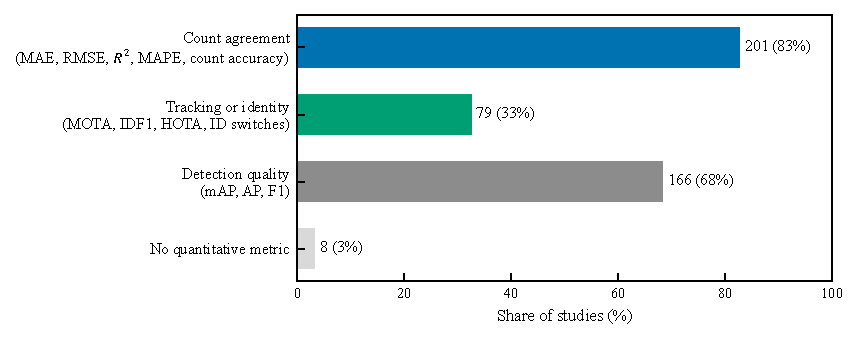
\includegraphics[width=0.62\textwidth]{F07_metrik}
\caption{Metric types reported by the multi-observation method studies, coded from the full text ($n=\nMethodMetric$).}\label{fig:metrik}
\end{figure*}

Where both were reported, identity and count metrics ranked the same trackers differently \citep{qi2025assessment,ishizuka2024eggplant}, so a ranking by count alone is provisional. Section~\ref{sec:agenda} answers the first two questions from this evidence and grades each finding (Table~\ref{tab:certainty}).

\section{Assigning one class to each fruit}\label{sec:class}

An inventory for selective harvesting needs the distribution of fruit among classes as well as the total. A ripe fruit assigned to the intermediate class changes two class counts and leaves the total unchanged. A missed immature fruit changes the immature count and the total. An association error can create both effects when one observation of a fruit forms a second record with a different label. The three types of error call for different measurements and different interventions.

\subsection{What per-image class results establish}

Single-image studies establish how well visible fruit can be distinguished under stated conditions. In \citet{deng2024detection}, a blueberry detector gave an RMSE of 10.39 fruit per test image and 3.62 percentage points for the proportion of ripe fruit. Dense clusters and poor focus contributed to misses. Transitional colours led to errors in the ripe share even when a berry was detected. The authors also flagged uncertainty in annotating the transitional berries. The two outcomes are complementary. A precise count of visible berries does not establish that the ripe share is correct.

Confusions are often concentrated where class boundaries require a decision about a continuous trait. For four tomato ripeness levels, \citet{pisharody2025precise} reported a true-positive rate of 0.627 for the intermediate level and 0.922--0.972 for the other levels in their test confusion matrix. For three classes of wild blueberries, \citet{maceachern2023detection} found the intermediate red class to have the lowest average precision at an intersection-over-union threshold of 0.50 in each of six networks. In \nKelasLainTengah of \nKelasLain reviewed image or detection results that reported at least three ordered maturity classes, an intermediate class performed worst. That pattern concerns the tested images and their class definitions. It does not identify the class with the greatest loss at plant level.

Classes need not refer to maturity. \citet{chiu2025remote} assigned size classes as well as ripeness classes in a scaled greenhouse validation setup. Their size results concern the fruit in that setup and give no evidence on repeat observations. \citet{soto2026monocular} estimated a distribution of grape berry diameters and a total berry count from one image of a bunch. Adding distance transforms derived from segmentation lowered the best validation count MAE from 5.9777 to 5.6659 berries. Their quantity model applied a correction to an initial segmented count and did not include a direct regression baseline. For a sorting or thinning decision, the distinction is whether a histogram predicts a quantity in each bin or an inventory records the bin of each observed berry. Tracking a particular berry across views requires individual records.

\subsection{Classification conditional on identity}

A class label can be carried from one detection, attached during linking, or assigned after several views support one identity. These choices determine where a disagreement goes. With class-gated linking, changing the class can terminate a valid track and create another record. With class assigned after linking, observations can disagree without changing the number of records, provided the linking is sound. \citet{kirk2021robust} pooled each track's previous observations as a cue for re-identifying strawberries, because the visible portion of a partly hidden fruit can imply a different maturity class.

Of the \nPerClass multi-observation studies that report per-class counts, \nClassUnstated did not specify how detections became one class per fruit. A class was carried by the tracker in \nClassDuring, assigned after tracking or in a fused model in \nClassAfter, or kept with each detection in \nClassPerDet. Only \nClassVote stated a vote or an averaging rule for disagreeing observations. The distinction matters even when a paper shows a tracked box with a class label. A sequence of classed boxes does not specify how the final record is counted.

Voting and averaging require the observations attached to an identity to be sufficiently informative. \citet{lin2026tomato} assigned the most frequent predicted class across the track. With annotated boxes, reported classification accuracy after voting ranged from 38\% to 81\% across datasets and classifiers. \citet{qi2024improved} used the modal maturity level of cherry-tomato clusters and reported 90.84\% maturity accuracy after excluding counting errors, alongside a count accuracy of 92.79\%. The maturity figure is conditional on the exclusions made in their evaluation. \citet{rong2025end} weighted cluster maturity observations by predicted occlusion. In the denser of two greenhouses, the system returned 87.1\% of the overall hand count of 202 clusters and 61.4\% for the 40--60\% maturity bin. Repeated observations can reduce frame-level fluctuations. The evidence remains limited when views expose the same atypical part of a fruit or when a group already contains observations of different fruit.

Fused geometry supplies another way to decide a label once. \citet{zhang2022measurement} registered two views of each of 50 greenhouse tomato plants and found fruit in the fused cloud with 86.19\% precision and 83.39\% recall against 277 reference fruit. The study also reported maturity classification accuracy of 96.09\% on separate image samples. The two results support different links in the pipeline. The image-sample score leaves open whether matched 3D fruit records carry the correct maturity labels.

\subsection{Measuring class error on unique fruit}

Write \(N_c\) for the number of visible reference fruit in class \(c\) and \(\widehat N_c\) for the predicted count. Match fruit to records before using class labels. Let \(I_c\) and \(O_c\) be the numbers of matched fruit transferred into and out of class \(c\), respectively. Let \(U_c\) count unmatched predictions assigned to \(c\) and \(L_c\) unmatched reference fruit of class \(c\). The signed error is
\begin{equation}
\widehat N_c - N_c = U_c - L_c + I_c - O_c.
\label{eq:class-flow}
\end{equation}
The transfer terms cancel across classes. In Fig.~\ref{fig:inventory-error}, the visible reference and the prediction each contain eight records. The ripe count nevertheless rises from three to four because D moves from unripe to ripe. If a class cannot be assigned reliably, recording it as unknown exposes the missing attribute while preserving the information that the fruit was found.

The same distinction appears in the observed inventories. \citet{ogundele2025real} reported MAPE of 9.52\% for the total strawberry count and 16.25\% for the semi-ripe count, the least reliable class in their test. \citet{wang2025tomato} reported a mean count error of 6.6\% for all tomatoes and 12.3\%, 16.9\%, and 17.3\% for the ripe, semi-ripe, and unripe classes. The weakest class was less accurate than the total in \nKelasLebih of \nKelasBanding comparable unique-fruit results. Among \nKelasUnik results for unique fruit with at least three ordered maturity classes, the least mature class was weakest in \nKelasUnikMentah and an intermediate class in \nKelasUnikTengah. In blueberry videos, \citet{wu2025maturity} found the lowest counting accuracy for green fruit (64.24\%, against 74.38\% for purple and 78.84\% for blue). The per-class pattern depends on the balance of misses and class transfers.

No multi-observation study in the class-count subset supplied a confusion matrix evaluated on matched unique fruit. Such a matrix, accompanied by missed and unmatched counts by class, would distinguish the class ambiguity that can be addressed by aggregating observations from the small or occluded fruit that require better acquisition or detection. For harvest classes, it should also state how reference labels were assigned and whether assessors agreed near the boundaries (Section~\ref{sec:agenda}).

\section{What depth contributes and where it fails}\label{sec:depth}

Depth can locate a fruit within the target row, describe the size of a partly occluded fruit, or provide coordinates for linking it across images. These are separate uses. A better segmentation mask or a more accurate diameter does not establish that two observations refer to the same fruit. The \nDepth supporting depth and 3D studies primarily address observation. Tests that ask whether depth resolves identity belong to the multi-observation evidence.

\subsection{Suppressing background without discarding fruit}

A range threshold can remove fruit behind the target row when the rows are well separated. \citet{afonso2020tomato} used depth to remove tomatoes in the row behind the one under observation. \citet{devanna2025yield} applied a comparable filter to images of 13 grapevines. Their estimate differed from the visual count in the same images by 12.2\% and from the post-harvest count by 33.9\%. The larger discrepancy against harvest reflects a broader target than the count visible in the same images. A range filter can reject fruit from another row, but leaves unseen bunches unobserved.

Requiring agreement between modalities can trade recall for precision. \citet{sun2022noise} compared five setups on the same outdoor fruit images. The red-green-blue (RGB) model gave an average precision at 0.50 intersection over union (AP50) of 94.1\%. Concatenating raw depth reduced it to 90.5\%, and requiring agreement between separate RGB and depth detectors raised precision from 89.8\% to 94.9\% while reducing recall from 92.2\% to 69.0\%. Their attention-based feature fusion reached AP50 of 95.4\% with recall of 94.1\%. The depth maps had holes. A missing depth value under a hard agreement rule can veto a true colour detection, whereas feature fusion can give the range cue less weight where it is unreliable.

Similar comparisons show why a sensor label is insufficient to describe an intervention. On peaches acquired with an Azure Kinect, \citet{luo2022multi} reported that adding depth to RGB reduced mean average precision (mAP) from 93.3\% to 92.7\% for unbagged fruit and from 72.4\% to 72.3\% for bagged fruit. On apples in 1{,}000 aligned RealSense images, \citet{kaukab2024improving} reported AP50 of 91.5\% for RGB and 92.5\% for concatenated RGB and raw depth. It reached 96.4\% after depth holes were filled and the background beyond 1~m was removed. On a cross-field and cross-day citrus test, \citet{liu2026geosphere} improved mAP averaged over intersection-over-union thresholds from 0.562 to 0.642 with gated depth fusion and geometry-aware rescoring. The valid depth fraction was lower in the denser of their two test fields. The larger gain belongs to the full method, which changed fusion and confidence estimates together.

A comparison that held detection and tracking fixed isolated the contribution of a depth filter. On 70 greenhouse tomato videos, \citet{zhang2024counting} reported 81.17\% count accuracy without a monocular depth filter and 83.87--93.80\% across seven thresholds. The best threshold was chosen using those same videos. The result supports the ability to remove some out-of-row detections on that material. It leaves open the threshold's error on new rows and how many true targets it discards. Comparing fusion systems also requires a control with the same network capacity and an uninformative or shuffled depth channel, so that changing the architecture and adding range information are separable.

\subsection{Reconstructing visible fruit and measuring size}

Two fruits at similar range can form one connected set of depth points. In Kinect imagery with 637 reference citrus fruit, \citet{lin2019field} reported F1 scores of 0.6950 for region growing and 0.6633 for Euclidean clustering. Their density clustering after a depth filter reached 0.9197. In peach point clouds, \citet{wu2019automatic} raised recall for touching fruit from 69.23\% to 89.74\% by fitting spheres. Recall for fruit obstructed by branches or leaves rose from 68.57\% to 74.29\%, a smaller gain than for touching fruit. These failures differ. A spatial grouping rule may separate touching fruit when samples exist for both surfaces. It cannot locate a fruit with no informative measurement.

Sizing introduces selection. \citet{genemola2023looking} inferred the hidden contour of partly occluded apples from colour and photogrammetric depth, using amodal segmentation, which estimates the full outline of a visible object. Their diameter MAE fell from 4.5 to 2.93~mm when the most occluded apples were discarded. The most restrictive visibility cutoff yielded the smallest error in validation, but a less restrictive cutoff better represented the size distribution. On a separate set of greenhouse tomato images, \citet{hao2024vision} could size 180 of 215 fruit. Most detection misses were fruit smaller than 15~mm, and 12 additional fruit were too occluded to measure. An error metric calculated only for fruit that could be sized omits those losses. For a class-wise inventory based on size, the size distribution and the fraction of fruit left unsized are both necessary.

\subsection{When range can resolve correspondence}

Depth supports association when measurements from two views can be compared in the same coordinate frame. \citet{wei2025multi} matched opposite sides of apple trees using a distance threshold of about one fruit diameter (70--85~mm). What matters for that decision is how distances between measurements of one fruit compare with distances between measurements of different fruit. A range error in a single image does not quantify the difference. Pose error, uncertainty in the position of a partially sampled fruit, and motion between captures all enter the registered coordinates.

A simple bound identifies what should be measured. If the registered positions each have error at most \(e\) and the minimum distance between distinct fruit centres is \(d\), a pair from one fruit can be up to \(2e\) apart. A pair from different fruit can be as close as \(d-2e\). A fixed distance threshold can separate all such pairs under these assumptions if \(d>4e\). This is a sufficient condition for an idealized static scene, rather than a crop-specific threshold. In practice, reporting the distributions of same-fruit and different-fruit distances by view separation is more informative than reporting a mean depth error alone.

Range noise increases with distance in sensor tests \citep{neupane2021evaluation}. On apple trees, \citet{fu2026mt} reported a pooled standard deviation of localization error of approximately 9.15~mm at 0.8~m and 14.14~mm at 1.6~m against a light detection and ranging (LiDAR) reference. Outdoor illumination is another source of failure. \citet{qureshi2023seeing} reported that sun glare degraded stereo matching and wind disrupted registration, whereas \citet{parr2023grape} obtained range images of grape bunches in direct sunlight with a smartphone time-of-flight sensor. For on-palm bunches, \citet{goh2025outdoor} used an acceptance band of \(\pm 20\)~cm at 3.0--4.0~m against tape measurements. That is a data-quality criterion. A proposed association threshold still requires measured residuals after registration and the spacing of neighbouring bunches (Section~\ref{sec:palm}).

\subsection{Predicted depth and physical scale}

Monocular depth can provide relative depth cues without active range sensing \citep{ranftl2021vision}. Its scale needs a reference for metric sizing or registration across independently processed images. On the PApple data, \citet{tan2025apple} reported mean absolute diameter errors of 4.02~mm with the provided depth and 10.99~mm with uncalibrated monocular depth. Calibration to known diameters reduced the latter to 9.09~mm with one global fit and 7.72~mm with an image-specific fit. The latter uses a stronger reference and cannot be extrapolated to images with no calibration measurement.

Converting depth predictions into spatial links adds uncertainties that a harvest count alone cannot distinguish. \citet{bellocchio2022novel} used predicted depth with estimated camera poses to merge detections on 18 mango trees. The mean absolute percentage error against harvest was reported as 33.80\%. Because the study did not vary depth alone, the result does not distinguish depth error from pose, detection, or clustering error. A relative-depth gate can be useful earlier in the pipeline, as in the tomato count above. Where the task is to match a bunch at widely separated viewpoints, a meaningful evaluation holds the detector fixed, reports registration quality, and compares predicted depth with measured depth and with a system using no range cue.

\section{Oil palm: from bunch grading to a census}\label{sec:palm}

A grader at a mill assigns a maturity class to a harvested bunch. A camera on a harvester locates a bunch and may estimate where to cut. A census of standing palms needs a count of unique bunches by maturity on each palm. Each task has a different reference and a different exposure to occlusion. The distinction explains why a high grading or detection score can coexist with an unresolved census problem. Of the \nPalm studies assigned to oil-palm imaging, \nPalmCls classified images of individual bunches and \nPalmDet detected bunches in a scene. \nPalmMill used mill, conveyor, or laboratory settings, and \nPalmOnTree specifically imaged bunches on the palm. The descriptive distribution is given in Supplementary Section~S8.

\subsection{What grading experiments establish}

Colour and texture can distinguish maturity when the bunch occupies the image and illumination is controlled. \citet{septiarini2021machine} obtained 98.3\% accuracy for three maturity levels using colour and texture features. Half-ripe and ripe bunches were confused where their colours were similar. \citet{phimpisan2023real} combined controlled ultraviolet excitation with image analysis of harvested Tenera bunches and reported full agreement with manual categorization under that setup. Neither comparison changes the view of a standing bunch or establishes the same reference classes as a preharvest census.

Detection experiments add spatial localization. On images assembled from Google and Kaggle, \citet{chen2022detection} reported mAP of 98.5\% at 31.8~ms for YOLOv4 and 96.4\% at 11.4~ms for YOLOv5. This is a speed and detection comparison within their image collection. The authors left testing in a plantation to future work. \citet{junos2021optimized} evaluated a detector for bunches, palms, and a harvester grabber in plantation imagery. The reported mAP was 98.68\% at an overlap threshold of 0.50 and 73.25\% averaged over thresholds from 0.50 to 0.95. Those values describe different localization criteria applied to the same task. The study proposed future work on video and counting.

\subsection{What changes when bunches remain on the palm}

Scores on grading videos depend on which classes and recording conditions the evaluation includes. In smartphone videos of harvested bunches, \citet{junior2023video} reported 97.64\% mAP50 for the best variant in their single-class test table and 70.21\% for the best variant in their mixed-class test table. The variants were configured differently, so this is not a controlled estimate of the effect of mixing classes. In grading piles of harvested bunches, \citet{suharjito2023real} reported high scores on a frame-level split, while deployment on new phone videos gave average F1 scores of 0.52--0.64 for quantized models. The new videos and quantization changed together. On standing palms, \citet{naftali2024palm} reported mAP50 of 75\% across five classes with plantation videos separated between training and testing. Their model reached 99.4\% on a separate harvested-bunch dataset. The settings and target instances differed, so the comparison identifies a transfer problem without isolating its causes.

The target and split are particularly important when interpreting an on-palm score. \citet{lai2022real} evaluated ripe-bunch detection on 20 palms in another area of an estate and reported mAP of 87.9\% for that one class. In SawitMVC, \citet{indriani2026sawitmvc} tested a deliberately untuned YOLO26m detector on 141 palms with four maturity classes. The reported overall AP50 was 53.1\%, with per-class values of 35.4--73.9\%. The least mature class, which contains small bunches, had the lowest AP50, and the dataset authors noted ambiguity between the two- and three-month classes. The one-class and four-class results set different evaluation targets. They provide no estimate of the number of duplicates when the same bunch is photographed around the palm.

\begin{figure*}[!t]
\centering
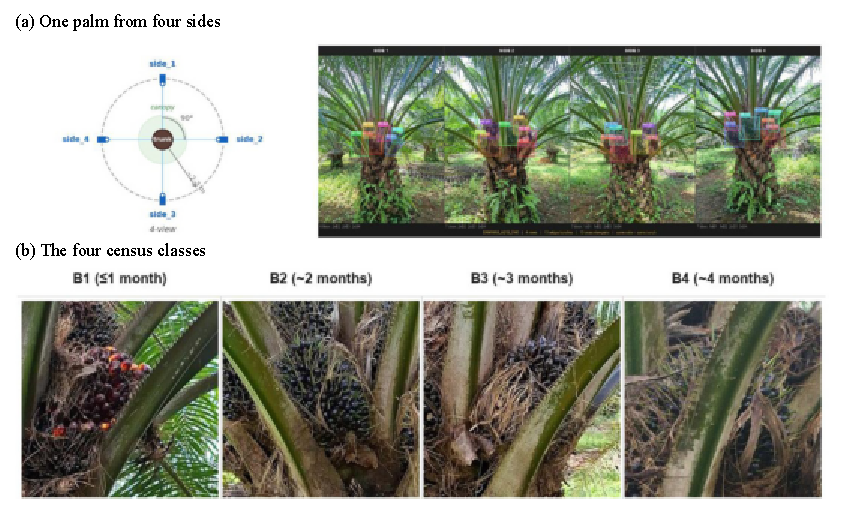
\includegraphics[width=\textwidth]{F11_foto_sawit}
\caption{Oil-palm census imagery in SawitMVC: (a) one palm photographed from four sides, with the boxes of one bunch drawn in the same colour in every photograph; (b) bunch crops of the four census classes, from at most one month (B1) to about four months (B4) before harvest. Adapted from \citet{indriani2026sawitmvc} under a CC BY 4.0 licence.}\label{fig:fotosawit}
\end{figure*}

Fig.~\ref{fig:fotosawit} shows why this is a correspondence problem. A bunch occupies different image locations in views around the trunk and fronds hide different parts from each direction. In SawitMVC, 25.4\% of annotated bunches were seen in only one photograph \citep{indriani2026sawitmvc}. Raising the required number of views for a valid record can remove false detections, but it would also discard genuine bunches that were visible once. Conversely, accepting every detection from every view creates duplicates. The classes with similar dark surfaces add little discrimination, so the class label is a weak candidate filter near a maturity boundary. For geometry, the registration residual at bunch height needs to be compared with the separation of neighbouring bunches (Section~\ref{sec:depth}). The stereo dataset of \citet{goh2025outdoor} supplies depth at field distances, without testing this matching decision.

\subsection{Where existing counts stop}

Counting on a conveyor and counting beneath a palm use different units and acquisition conditions from a census of standing bunches. \citet{shiddiq2023counting} and \citet{aji2021automatic} tracked harvested bunches over a conveyor, where motion imposes a predictable ordering. \citet{daud2022loose} and \citet{daud2023detection} tracked the palm and used a summary of per-frame counts of loose fruit below it. Tracking the palm identifies the unit of aggregation. The individual loose fruit still have no cross-frame identities. \citet{kassim2012oil} linked repeated photographs of marked bunches by physical tags. \citet{warni2026stereo} matched loose-fruit detections in the two images of a stereo pair over 20--120~cm, a useful local correspondence test with a much smaller baseline and range than the multi-side palm census. The video data of \citet{suharjito2025oil} were acquired around palms but the released boxes do not link detections between frames. In the reports retrieved for this review, these results leave automatic linking of on-palm bunches across independently captured sides unresolved.

\subsection{What SawitMVC can test}

Both authors of this review co-authored SawitMVC \citep{indriani2026sawitmvc}. The published dataset contains 18{,}540 boxes for 9{,}823 bunches on 953 palms, with four to eight photographs per palm. The linked boxes provide a visible-identity reference, and each reference bunch has a census class. On 141 test palms, the published baselines show how much a count can improve without establishing correspondence.

\begin{table*}[!t]
\centering
\caption{Published SawitMVC count baselines on 141 test palms.}\label{tab:palm-baselines}
\small
\begin{tabularx}{\textwidth}{@{}L{3.2cm}YL{3.15cm}L{3.35cm}@{}}
\toprule
Input & Count rule & Class counts within one bunch (\%) & Palms with all four within one (\%)\\
\midrule
Annotated boxes & Sum across views & 50.00 & 6.38\\
Annotated boxes & Divide by training-set duplication ratio & 95.57 & 86.52\\
Annotated boxes & Support vector regression on view counts & 96.81 & 88.65\\
Detector boxes & Divide by the same ratio & 72.34 & 30.50\\
Detector boxes & Support vector regression on view counts & 75.35 & 33.33\\
\bottomrule
\end{tabularx}

\smallskip
\parbox{\textwidth}{\rmfamily\footnotesize\textit{Note:} The reference includes bunches annotated in at least one image. For each class, accuracy is the fraction of palms within one bunch of the reference. Class accuracy averages those four fractions. Palm accuracy is the fraction of palms meeting the tolerance in all four classes.}
\end{table*}

Dividing the annotated box counts by the fitted duplication ratio of 1.89 gave a mean class accuracy of 95.57\% within one bunch of the annotated reference (Table~\ref{tab:palm-baselines}). Support vector regression increased the mean to 96.81\%. Neither method decides which boxes belong to the same bunch. The tolerance is also lenient for classes with low counts. With the detector replacing annotated boxes, the mean signed error of the ratio method rose from \(+0.009\) to \(+0.381\) bunches per palm and class. The ratio was fitted to annotation counts and held fixed when applied to predictions. The difference therefore combines detection errors with any mismatch between the ratio and detector outputs. Refitting the ratio on detector outputs from training palms would make a comparison with an association method more informative.

The next experiment can separate what the detector finds from what the matcher links. On the existing test palms, a correspondence method can first receive the annotated boxes and be assessed for splits and merges, then receive detector boxes and be assessed for the complete inventory. The count baselines should be fitted on the training palms under each input condition. The four classes should be evaluated after matching, with a unique-bunch confusion matrix and misses by class. Holding out a plantation can probe transfer across the available sites. A broader claim about a full census additionally needs new palms and a field reference that includes bunches hidden from all photographs.

\section{Discussion}\label{sec:agenda}

The intended output determines how much evidence a counting system needs. A calibrated count can serve a load forecast where the relationship between visible fruit and harvest holds on new plants. A system that must revisit, selectively harvest, or audit individual fruit needs persistent records. In that case the capture geometry determines which correspondence cues are available, and the reference determines which errors can be measured. The following implications apply across the crops reviewed, with oil palm illustrating the discrete-view case.

\subsection{Choose the capture and association together}

For continuous video, overlapping frames give a practical basis for motion-based tracking. A tracker can preserve identity only while its prediction remains useful across a gap in observations. On 10-frame/s mango video, a 15-frame lifetime gave a lost track about 1.5~s to recover \citep{wang2019mango}. In the 110-frame test clip, the reported 9.9\% duplicate rate and 7.3\% miss rate yielded a net overcount of about 2.6\%. A field trial should reproduce the actual walking or vehicle speed and report association outcomes by occlusion gap. Reporting the lifetime in seconds as well as frames makes it possible to compare tests at different frame rates.

Separate passes and photographs from fixed positions offer little temporal continuity. In these conditions, spatial registration or a correspondence model evaluated on linked identities can supply candidate matches. A geometric gate can reduce the candidate set before appearance decides among nearby fruit, subject to the separation condition discussed in Section~\ref{sec:depth}. For coarse scans or weak calibration, reporting a set of unresolved pairs or an uncertainty interval may better reflect the available evidence than forcing a match. The apple comparison in Table~\ref{tab:assoc} shows that 3D merging can improve opposite-side counts on shared data. It does not establish a distance threshold for bunches high in an oil-palm canopy.

Video studies have compared tracking algorithms, counting rules, and frame rates using reference tracks or counts (Table~\ref{tab:assoc} and Section~\ref{sec:mech-track}). Between independently acquired views, tests need annotations of which fruit correspond across the views. Outside agriculture, \citet{ristani2018features} trained appearance features for multi-camera person tracking using examples selected for their difficulty. \citet{he2021transreid} evaluated explicit camera and viewpoint information on person and vehicle benchmarks. A corresponding fruit benchmark would label the difficult pairs directly, especially where neighbouring fruit share the same class and have similar visible surfaces.

\subsection{What the evidence supports across studies}

Linking repeated observations often moved counts closer to their references where the same fruit appeared more than once (Table~\ref{tab:certainty}). The tracker comparisons were sensitive to the counting rule and to whether the outcome measured track accuracy or count error. Each result applies to the tested detector, acquisition, and reference. Testing several methods on the same orchard images helps isolate differences between methods. Testing them on independent orchards addresses transfer.

The studies also distinguish three reasons a method may appear better. Better acquisition exposes more distinct fruit. Better observation detects more of the visible fruit and rejects spurious detections in the same views. Better association recovers the identities among a fixed set of observations. A pipeline can improve the count through any of them. The 3D correction in \citet{liu2018robust}, for example, rejected distant or unusual detections as well as duplicate tracks. The paired result measures the combined effect of removing outliers and linking duplicate tracks. The class results similarly show why changes to maturity weights should be assessed with a fixed correspondence, followed by a separate test of coupling class and identity.

%% Dibuat otomatis oleh tools/scopus/tabel_lampiran.py dari kepastian_klaim.tsv; jangan disunting manual.
\begin{table*}[!t]
\caption{Certainty of the main findings, graded from the comparisons on the same data that bear on each finding.}\label{tab:certainty}
\footnotesize
\setlength{\tabcolsep}{3pt}
\begin{tabularx}{\textwidth}{@{}X*{8}{>{\centering\arraybackslash}p{1.15cm}}l@{}}
\toprule
Finding & \hspace{0pt}Comparisons & Studies & Groups & Crops & Field reference & Other method favoured & Mixed & Against & Certainty\\
\midrule
Linking observations moved the count towards the reference; one view per side undercounted and summing overcounted & 12 & 12 & 10 & 5 & Yes & Yes & 2 & 0 & High \\
\addlinespace[2pt]
Which tracker family ranked first changed between studies and between identity and count metrics & 15 & 15 & 13 & 6 & Yes & Yes & 0 & 0 & High \\
\addlinespace[2pt]
A generic appearance descriptor helped mainly when detections went missing & 3 & 3 & 3 & 2 & No & Yes & 0 & 2 & Low \\
\addlinespace[2pt]
The rule used to count tracks changed how tracking pipelines ranked by count error & 3 & 3 & 3 & 3 & No & No & 0 & 0 & Moderate \\
\addlinespace[2pt]
Changing from a counting line to an alternative rule reduced error more than changing the upstream pipeline & 2 & 2 & 2 & 2 & No & No & 1 & 1 & Low \\
\addlinespace[2pt]
A geometric or 3D step after tracking or summation removed duplicates, including the second side of a row & 10 & 10 & 7 & 3 & Yes & No & 3 & 0 & Moderate \\
\addlinespace[2pt]
A statistical correction was accurate where it was fitted and lost accuracy elsewhere & 5 & 4 & 3 & 3 & Yes & No & 2 & 0 & Moderate \\
\addlinespace[2pt]
A descriptor built for the fruit improved the tracker & 10 & 10 & 10 & 5 & No & No & 2 & 1 & Moderate \\
\addlinespace[2pt]
Depth used to remove background or far-row fruit brought tracked counts closer to the reference & 7 & 7 & 6 & 3 & Yes & No & 0 & 1 & Moderate \\
\addlinespace[2pt]
A lower frame rate lowered tracking accuracy & 3 & 3 & 3 & 2 & No & Yes & 0 & 0 & Moderate \\
\addlinespace[2pt]
Adding views or frames did not lower the count error consistently & 9 & 9 & 9 & 6 & Yes & No & 2 & 3 & Low \\
\bottomrule
\end{tabularx}

\smallskip
\parbox{\textwidth}{\textit{Note:} A comparison is counted once for each finding it bears on. Groups, studies from one research group or on the same data, counted once. Field reference, at least one supporting comparison used a harvest, packhouse, or hand count on the plant. Other method favoured, at least one supporting comparison favoured a method that was not the authors' own. Mixed and Against, comparisons whose result was mixed or opposed the finding. Certainty: High, at least three supporting groups and two crops, no group against, a field reference, and another method favoured; Moderate, at least two supporting groups and none against, or at least three supporting groups and one against; Low, otherwise.}
\end{table*}


\subsection{Position relative to earlier reviews}\label{sec:position}

Earlier reviews supply three bodies of evidence that this synthesis brings together. Detector-centred reviews explain small objects, dense overlap, variable backgrounds, and limited labels \citep{koirala2019deepb,gong2025fruit}. Reviews of yield estimation place an image count alongside destructive sampling, remote sensing, and statistical forecasting \citep{anderson2021technologies,he2022fruit,trentin2024tree}. Oil-palm reviews describe sensing and classification of bunch maturity and identify difficulties in deployment \citep{lai2023oil,goh2025fresh,nordin2026systematic}. These accounts explain why detection can improve, why field calibration matters, and why a grading result is difficult to transfer. Section S10 of the supplement compares the scope of the closest reviews.

The acquisition design determines which cues a system can use to link fruit observations. \citet{miranda2023fruit} distinguished tracking in video from association in 3D. This review extends that distinction by identifying the capture conditions under which each cue can resolve a repeated observation. For example, rapid and continuous views permit a motion model, whereas opposite sides may need a shared geometric frame. The synthesis also distinguishes yield calibration, matching detections, and assigning classes. Success at one step cannot establish the accuracy of the next. In the earlier reviews represented in the comparison, the assignment of one class after linking across discrete views remains unaddressed. That gap matters for selective harvest because the output is a set of classified fruit on named plants.

\subsection{Experiments that would resolve the main uncertainties}\label{sec:experiments-review}

\textit{(i) Identify where an inventory fails.} Collect an independent field or harvested reference on a subset of plants and link all visible instances across the acquired views. Evaluate the same predictions against both references on those plants. Equation~\ref{eq:count-gap} shows how the difference separates incomplete coverage from errors among visible fruit. Report unmatched fruit and predictions, and report splits and merges under annotated inputs. A correct row total can otherwise conceal errors of opposite sign within a plant and between neighbouring plants.

\textit{(ii) Compare mechanisms on a common candidate set.} Hold the observations and plant boundaries fixed. Compare an unlinked sum, a correction fitted on training plants, and feasible linking mechanisms, including tracking or geometric association where the acquisition permits them. Hold the counting rule fixed, or test every tracker under every rule if their interaction is of interest. Report the resulting plant counts and the recovery of unique identities. This design would distinguish the value of the matcher from changes to the detector, calibration divisor, or track filtering rule.

\textit{(iii) Measure class assignment after association.} With reference identities fixed, compare a label from one representative view with a vote or weighted estimate across views. Measure transfers among classes and the rate of unknown labels. Then use the same observations to test whether class-gated linking changes splits and merges relative to linking without class constraints. Reference labels near ordered maturity boundaries should be checked by independent assessors. Equation~\ref{eq:class-flow} shows why total count error cannot substitute for this evaluation.

\textit{(iv) Test wide view gaps and changing geometry.} For each plant, subsample the same capture to compare known view separations, degrees of overlap, and object scales. Report matches and misses by these strata, with independent measurements of pose quality and depth validity. A useful result would show at which view separations a fixed geometric gate admits too many neighbouring fruit or rejects repeated observations of the same fruit. A revisit should record genuine changes in the population, including harvest or fruit loss, before those changes are counted as tracking failures.

\textit{(v) Test oil-palm transfer at the plant level.} Use the published visible identities and class counts from SawitMVC to compare association and aggregate correction on the same palms. Hold out a plantation before choosing thresholds and collect an independent set in another season to test temporal transfer. On a subsample, make a complete manual field count and reconcile visible reference bunches with it. That extra reference is necessary before making claims about a census of all bunches in a canopy.

\subsection{A minimum reporting set}\label{sec:reporting-set}

\begin{table*}[!t]
\centering
\caption{Measurements needed to interpret a reported fruit count.}\label{tab:reporting}
\small
\begin{tabularx}{\textwidth}{@{}L{2.7cm}YY@{}}
\toprule
Stage & Record or measurement & Inference it supports\\
\midrule
Acquisition & Plant or row unit, viewpoint spacing, overlap, frame rate and speed, season, count of reference fruit newly visible per view & Coverage gained with each view and scope for transfer to the intended protocol\\
Observation & Precision and recall on held-out plants, by occlusion, size, and class. Valid range data and measurement error where used & Whether a missed count begins with a missing, ambiguous, or misplaced detection\\
Association & Shared observations or fixed detector, linked identity reference, splits and merges by view gap, and performance on separate passes & Whether linking recovers identities and where continuity or registration fails\\
Attribute & One reference class per fruit, rule for disagreeing observations, matched confusion matrix, unknown labels and class-specific misses & Which class errors arise from label transfer and which arise from lost fruit\\
Inventory & Visible and field references for the same plant where possible, signed and absolute errors per plant and class, and the aggregation scale & Whether the result supports a visible inventory, a whole-plant estimate, or an aggregate forecast\\
\bottomrule
\end{tabularx}
\end{table*}

Table~\ref{tab:reporting} states the minimum needed to interpret a reported number. The unit must be kept consistent from acquisition to reference. Video annotation supports an estimate for visible fruit in the sequence. A packhouse reference supports a reconciled block total. A study can report an inventory result alongside a load estimate, provided that it describes their different references. Runtime should cover capture and association as well as the detector, particularly when a 3D reconstruction is compared with a single pass.

\section{Limitations of this review}\label{sec:limits}

The map is limited by database coverage and access to full texts. Scopus was the sole database. Full texts were unavailable for \nNotRetrieved of \nSought reports sought. Of those provisionally classified by topic, \nNotRetrievedMulti concerned multi-observation methods and \nNotRetrievedPalm oil-palm imaging. Missing reports also include \nNotRetrievedSingle single-view studies, \nNotRetrievedClass studies of class-specific counts, \nNotRetrievedDepth studies of depth or non-RGB imaging, \nNotRetrievedReview earlier reviews, and \nNotRetrievedTransfer transferable methods. The resulting gaps are more likely to affect the breadth of the supporting and oil-palm evidence than the set of retrieved multi-observation reports. The search retained a purposive subset of papers outside agriculture, so those papers illustrate transferable ideas without mapping their source fields.

One reviewer used a large language model for screening and coding, including the blinded second pass, and the independent checks of model results covered samples. Agreement on the blind human samples was \(\kappa=\kHumTitles\) for title decisions and \(\kappa=\kHumElig\) for eligibility codes. In the sample of \nSampleTitles title exclusions, \nSampleTitlesEligible were eligible after review of their abstracts. The exclusions from the two core query sets were rechecked, but the title exclusions in the other sets were not reviewed in full. The descriptive keyword codes for supporting groups were spot-checked. An unobserved method may therefore be missing from the search or from the available reports. Comparisons within one study still need to be interpreted within that study's own reference and design.

The analysis uses the outcomes reported by the primary studies. A favourable comparison with an author-developed baseline may reflect model choice, tuning, and test selection as well as the component under study. Use of the same public data by several publications limits independent confirmation. A count against imagery omits fruit never seen, a metric on annotated detections bypasses observation errors, and a randomized image split can retain similar views of one plant in training and evaluation. These tests quantify performance on different targets. The review interpreted the comparisons in relation to their references. It did not pool performance values or formally assess reporting bias.

\section{Conclusions}\label{sec:conclusion}

The effect of another view depends on which fruit it reveals and which it repeats. In dense mango canopies, counts from tracked video captured a larger share of the harvest than counts from two snapshots \citep{wang2019mango}. In thin orange canopies, summing four views tended to overestimate the crop because the same fruit appeared again \citep{mirhaji2021fruit}. Calibration can yield a usable forecast when the relationship between image and field counts holds on new plants. For an inventory, the system must decide which observations belong to each fruit. The ability to build those records depends on the capture protocol and the cues it provides for matching.

In video, short gaps can be bridged when the motion model or appearance cues keep a track distinguishable from its neighbours. The resulting count also depends on which tracks are accepted as records. Holding the detector and counting rule fixed makes a comparison of trackers interpretable. Across separate sides, a shared spatial frame can reduce repeated counts when registration is accurate relative to the distance between neighbouring fruit. A test of learned correspondence must likewise cover the view separations and occlusions it will face. In both cases, linked reference observations are needed to distinguish a correctly recovered identity from a count that happens to agree.

A class-wise inventory needs a decision about each recovered fruit when its views suggest different labels. A missed fruit reduces the count of its class. A label error transfers one fruit between two classes and leaves the total unchanged. In oil palm, linked bunch annotations across separately photographed sides provide a reference for testing these errors. The published count baselines estimate visible bunch totals by maturity. A direct test of correspondence would show whether particular bunches were recovered, while a field census on the same palms would establish how many bunches remain unseen.

The next comparisons should measure (i) coverage against an independent field count on the imaged plants, (ii) split and merged identities under shared observation inputs, and (iii) class confusion on matched fruit alongside misses by class. Repeating these comparisons across (iv) view separations and registration errors and (v) plantations and seasons would show where a method transfers. Reporting errors per plant and per class makes the results interpretable at the scale of a harvest decision. An estate total can hide omissions concentrated on particular palms or an overestimate of bunches ready to harvest.

\section*{CRediT authorship contribution statement}
\textbf{Muhammad Zainal Muttaqin}\par
Conceptualization, Methodology, Software, Data curation, Formal analysis, Investigation, Visualization, Writing -- original draft.

\textbf{Fatma Indriani}\par
Conceptualization, Methodology, Validation, Supervision, Project administration, Writing -- review \& editing.

\section*{Declaration of competing interest}
The authors declare that they have no known competing financial interests or personal relationships that could have appeared to influence the work reported in this paper. Both authors co-authored the SawitMVC dataset \citep{indriani2026sawitmvc}, which this review cites as the one oil-palm dataset that links bunches across views.

\section*{Funding}
\authorcheck{Funding information to be confirmed by the authors.}

\section*{Acknowledgements}
\authorcheck{Authors to complete, or delete this section if there is no one to acknowledge.}

\section*{Data availability}
Appendix~\ref{app:queries} provides the search strings. The Supplementary Material describes screening and coding and provides the full comparison register. Supplementary Data S1 lists all included reports and all reports excluded at full text, with reasons. The screening decisions, coded evidence, verification log, and analysis scripts accompany the review data. \authorcheck{Confirm the repository and add its DOI or link before submission.}

\section*{Declaration of generative AI and AI-assisted technologies in the writing process}
Large language models were used to assist with screening and coding (Claude, Anthropic), and with drafting, revision, and checking evidence against the cited sources (Claude, Anthropic, and Codex, OpenAI). The authors are responsible for reviewing and verifying the manuscript and its sources before submission.
